\chapter{Density functional theory as a screening method for dense metal membranes}

\section{Abstract}

\section{Introduction}
High impurity resistant dense metal membranes are being developed for hydrogen impurity enrichments of HRS samples with hydrogen derived from biomass, hydrocarbon or electrolysis. Metal membranes operate by selectively dissociating hydrogen, which then allows the hydrogen atoms to solubilize and subsequently permeate through the bulk of the separation layer. The problem is that many hydrogen impurities are also capable of adsorbing onto and interacting with the surface of many of the metals which comprise dense metal membranes. The impact of this adsorption can vary depending the molecule, Carbon monoxide for example will simply adsorb onto the surface and result in competitive adsorption between the hydrogen and impurity. Sulphur containing impurities which are commonly found in hydrocarbon sources and therefore are potentially present in any hydrogen produced from these methods. Sulphur containing impurities present more of a problem since they can potentially react with many metals used for hydrogen separation membranes. The impact of these contaminants can be minimized by designing alloy compositions that have a weaker attraction to the membrane, and therefore will have less of an affect at higher temperatures where these membranes operate.

Physically testing each potential membrane composition would be time consuming and costly due to the high price of palladium, the time required to synthesise specific membrane compositions, and performing the tests. Simulations provide a solution to this, allowing potential alloys to be screened for their interaction strength with each individual ISO 14687-2 impurity quickly, avoiding the cost of manufacturing each alliy composition. 

This chapter will calculate the behaviour of 14 palladium alloy composition under 13 ISO 14687-2 impurities. This is done by comparing the total energy of different configurations after relaxation of internal forces in the system. The close packed surfaces of palladium alloys were simulated as 

\section{Results and discussion}


\begin{table}[]
    \centering
    \caption{Simulated total energy values of ISO 14687-2 impurities}
    \label{gases}
    \begin{tabular}{@{}cc@{}}
    \toprule
    Gas          & \begin{tabular}[c]{@{}c@{}}Total Energy\\ $(kJ \times 10^{-21})$\end{tabular} \\ \midrule
    H            & -2.01                                                               \\
    N\textsubscript{2}           & -123.91                                                             \\
    O\textsubscript{2}           & -180.86                                                             \\
    CO           & -130.93                                                             \\
    CO\textsubscript{2}          & -221.95                                                             \\
    NH\textsubscript{3}          & -1933.22                                                            \\
    Ar           & -208.10                                                             \\
    CH\textsubscript{4}          & -50.73                                                              \\
    Formaldehyde & -136.13                                                             \\
    Formic Acid  & -227.08                                                             \\
    H\textsubscript{2}S          & -150.36                                                             \\
    He           & -12.62                                                              \\
    H\textsubscript{2}O          & -95.99                                                              \\ \bottomrule
    \end{tabular}
\end{table}

\subsection{Stability of palladium alloy compositions}
Hydrogen adsorption on the surface of palladium is a key value for the purpose of this experiment. The affinity for a palladium alloy to adsorb on the surface is the initial step for hydrogen permeation, and below a certain thickness becomes the rate limiting step. As expected all alloys had an affinity for hydrogen adsorption and these values matched what is generally found in literature. These values will be compared to the adsorption energies of other impurities on the alloys in order to determine their resistance to the impurity. The adsorption energies of hydrogen on a the Pd slab system is shown in figure \ref{Pdsite}. In a Pd system hydrogen preferentially adsorbs on the FCC and top sites at relativley even energies. At both of these sites hydrogen is able to form a stable system without being affected by other forces. HCP and top sites have a  lower affinity for hydrogen adsorption and this is likely due to the influence of competition by neighbouring sites which can provide higher stability.
Hydrogen adsorption on the surface of palladium is a key value for the purpose of this experiment. The affinity for a palladium alloy to adsorb on the surface is the initial step for hydrogen permeation, and below a certain thickness becomes the rate limiting step. As expected all alloys had an affinity for hydrogen adsorption and these values matched what is generally found in literature. These values will be compared to the adsorption energies of other impurities on the alloys in order to determine their resistance to the impurity. The adsorption energies of hydrogen on a the Pd slab system is shown in figure \ref{Pdsite}. In a Pd system hydrogen preferentially adsorbs on the FCC and top sites at relativley even energies. At both of these sites hydrogen is able to form a stable system without being affected by other forces. HCP and top sites have a  lower affinity for hydrogen adsorption and this is likely due to the influence of competition by neighbouring sites which can provide higher stability.
Hydrogen adsorption on the surface of palladium is a key value for the purpose of this experiment. The affinity for a palladium alloy to adsorb on the surface is the initial step for hydrogen permeation, and below a certain thickness becomes the rate limiting step. As expected all alloys had an affinity for hydrogen adsorption and these values matched what is generally found in literature. These values will be compared to the adsorption energies of other impurities on the alloys in order to determine their resistance to the impurity. The adsorption energies of hydrogen on a the Pd slab system is shown in figure \ref{Pdsite}. In a Pd system hydrogen preferentially adsorbs on the FCC and top sites at relativley even energies. At both of these sites hydrogen is able to form a stable system without being affected by other forces. HCP and top sites have a  lower affinity for hydrogen adsorption and this is likely due to the influence of competition by neighbouring sites which can provide higher stability.


\begin{table}[]
    \centering
    \caption{Simulated total energy values of alloy slabs}
    \label{slabs}
    \begin{tabular}{@{}cccc@{}}
    \toprule    
    Alloy/Metal Composition      & \begin{tabular}[c]{@{}c@{}}Total Energy\\ (ry)\end{tabular} & Total Energy (kJ) \\ \midrule
    Pd                       & -6653.38                                      & $-1.45\times10^{-17}$     \\
    PdAg\textsubscript{23}                   & -6774.37                                      & $-1.48\times10^{-17}$    \\
    PdAu\textsubscript{10}                   & -7545.53                                      & $-1.64\times10^{-17}$     \\
    PdAu\textsubscript{20}                   & -8437.613                                     & $-1.84\times10^{-17}$     \\
    Pd\textsubscript{60}Cu\textsubscript{40}                 & -5703.15                                      & $-1.24\times10^{-17}$     \\
    Pd\textsubscript{80}Cu\textsubscript{20}                 & -6178.29                                      & $-1.35\times10^{-17}$     \\
    Pd\textsubscript{70}Au\textsubscript{20}Zr\textsubscript{10}             & -8389.61                                      & $-1.83\times10^{-17}$     \\
    Pd\textsubscript{70}Cu\textsubscript{20}Zr\textsubscript{10}             & -6130.29                                      & $-1.34\times10^{-17}$     \\
    Pd\textsubscript{70}Ag\textsubscript{10}Zr\textsubscript{20}             & -6605.75                                      & $-1.44\times10^{-17}$     \\
    PdZr\textsubscript{10}                   & -6605.45                                      & $-1.44\times10^{-17}$     \\
    PdZr\textsubscript{20}                   & -6557.46                                      & $-1.43\times10^{-17}$     \\
    Pd\textsubscript{70}Au\textsubscript{20}Ag\textsubscript{10}             & -8485.99                                      & $-1.84\times10^{-17}$     \\
    Pd\textsubscript{70}Au\textsubscript{20}Cu\textsubscript{10}             & -8200.05                                      & $-1.79\times10^{-17}$     \\
    Pd\textsubscript{70}Cu\textsubscript{20}Ag\textsubscript{10}             & -6226.71                                      & $-1.36\times10^{-17}$     \\ \bottomrule
    \end{tabular}
    \end{table}
    Hydrogen adsorption on the surface of palladium is a key value for the purpose of this experiment. The affinity for a palladium alloy to adsorb on the surface is the initial step for hydrogen permeation, and below a certain thickness becomes the rate limiting step. As expected all alloys had an affinity for hydrogen adsorption and these values matched what is generally found in literature. These values will be compared to the adsorption energies of other impurities on the alloys in order to determine their resistance to the impurity. The adsorption energies of hydrogen on a the Pd slab system is shown in figure \ref{Pdsite}. In a Pd system hydrogen preferentially adsorbs on the FCC and top sites at relativley even energies. At both of these sites hydrogen is able to form a stable system without being affected by other forces. HCP and top sites have a  lower affinity for hydrogen adsorption and this is likely due to the influence of competition by neighbouring sites which can provide higher stability.
    Hydrogen adsorption on the surface of palladium is a key value for the purpose of this experiment. The affinity for a palladium alloy to adsorb on the surface is the initial step for hydrogen permeation, and below a certain thickness becomes the rate limiting step. As expected all alloys had an affinity for hydrogen adsorption and these values matched what is generally found in literature. These values will be compared to the adsorption energies of other impurities on the alloys in order to determine their resistance to the impurity. The adsorption energies of hydrogen on a the Pd slab system is shown in figure \ref{Pdsite}. In a Pd system hydrogen preferentially adsorbs on the FCC and top sites at relativley even energies. At both of these sites hydrogen is able to form a stable system without being affected by other forces. HCP and top sites have a  lower affinity for hydrogen adsorption and this is likely due to the influence of competition by neighbouring sites which can provide higher stability.
    Hydrogen adsorption on the surface of palladium is a key value for the purpose of this experiment. The affinity for a palladium alloy to adsorb on the surface is the initial step for hydrogen permeation, and below a certain thickness becomes the rate limiting step. As expected all alloys had an affinity for hydrogen adsorption and these values matched what is generally found in literature. These values will be compared to the adsorption energies of other impurities on the alloys in order to determine their resistance to the impurity. The adsorption energies of hydrogen on a the Pd slab system is shown in figure \ref{Pdsite}. In a Pd system hydrogen preferentially adsorbs on the FCC and top sites at relativley even energies. At both of these sites hydrogen is able to form a stable system without being affected by other forces. HCP and top sites have a  lower affinity for hydrogen adsorption and this is likely due to the influence of competition by neighbouring sites which can provide higher stability.


\subsection{Hydrogen and Impurity adsorption on palladium alloy membranes}
\subsubsection{Hydrogen}
Hydrogen adsorption on the surface of palladium is a key value for the purpose of this experiment. The affinity for a palladium alloy to adsorb on the surface is the initial step for hydrogen permeation, and below a certain thickness becomes the rate limiting step. As expected all alloys had an affinity for hydrogen adsorption and these values matched what is generally found in literature. These values will be compared to the adsorption energies of other impurities on the alloys in order to determine their resistance to the impurity. The adsorption energies of hydrogen on a the Pd slab system is shown in figure \ref{Pdsite}. In a Pd system hydrogen preferentially adsorbs on the FCC and top sites at relativley even energies. At both of these sites hydrogen is able to form a stable system without being affected by other forces. HCP and top sites have a  lower affinity for hydrogen adsorption and this is likely due to the influence of competition by neighbouring sites which can provide higher stability.

\begin{figure}
  \centering
  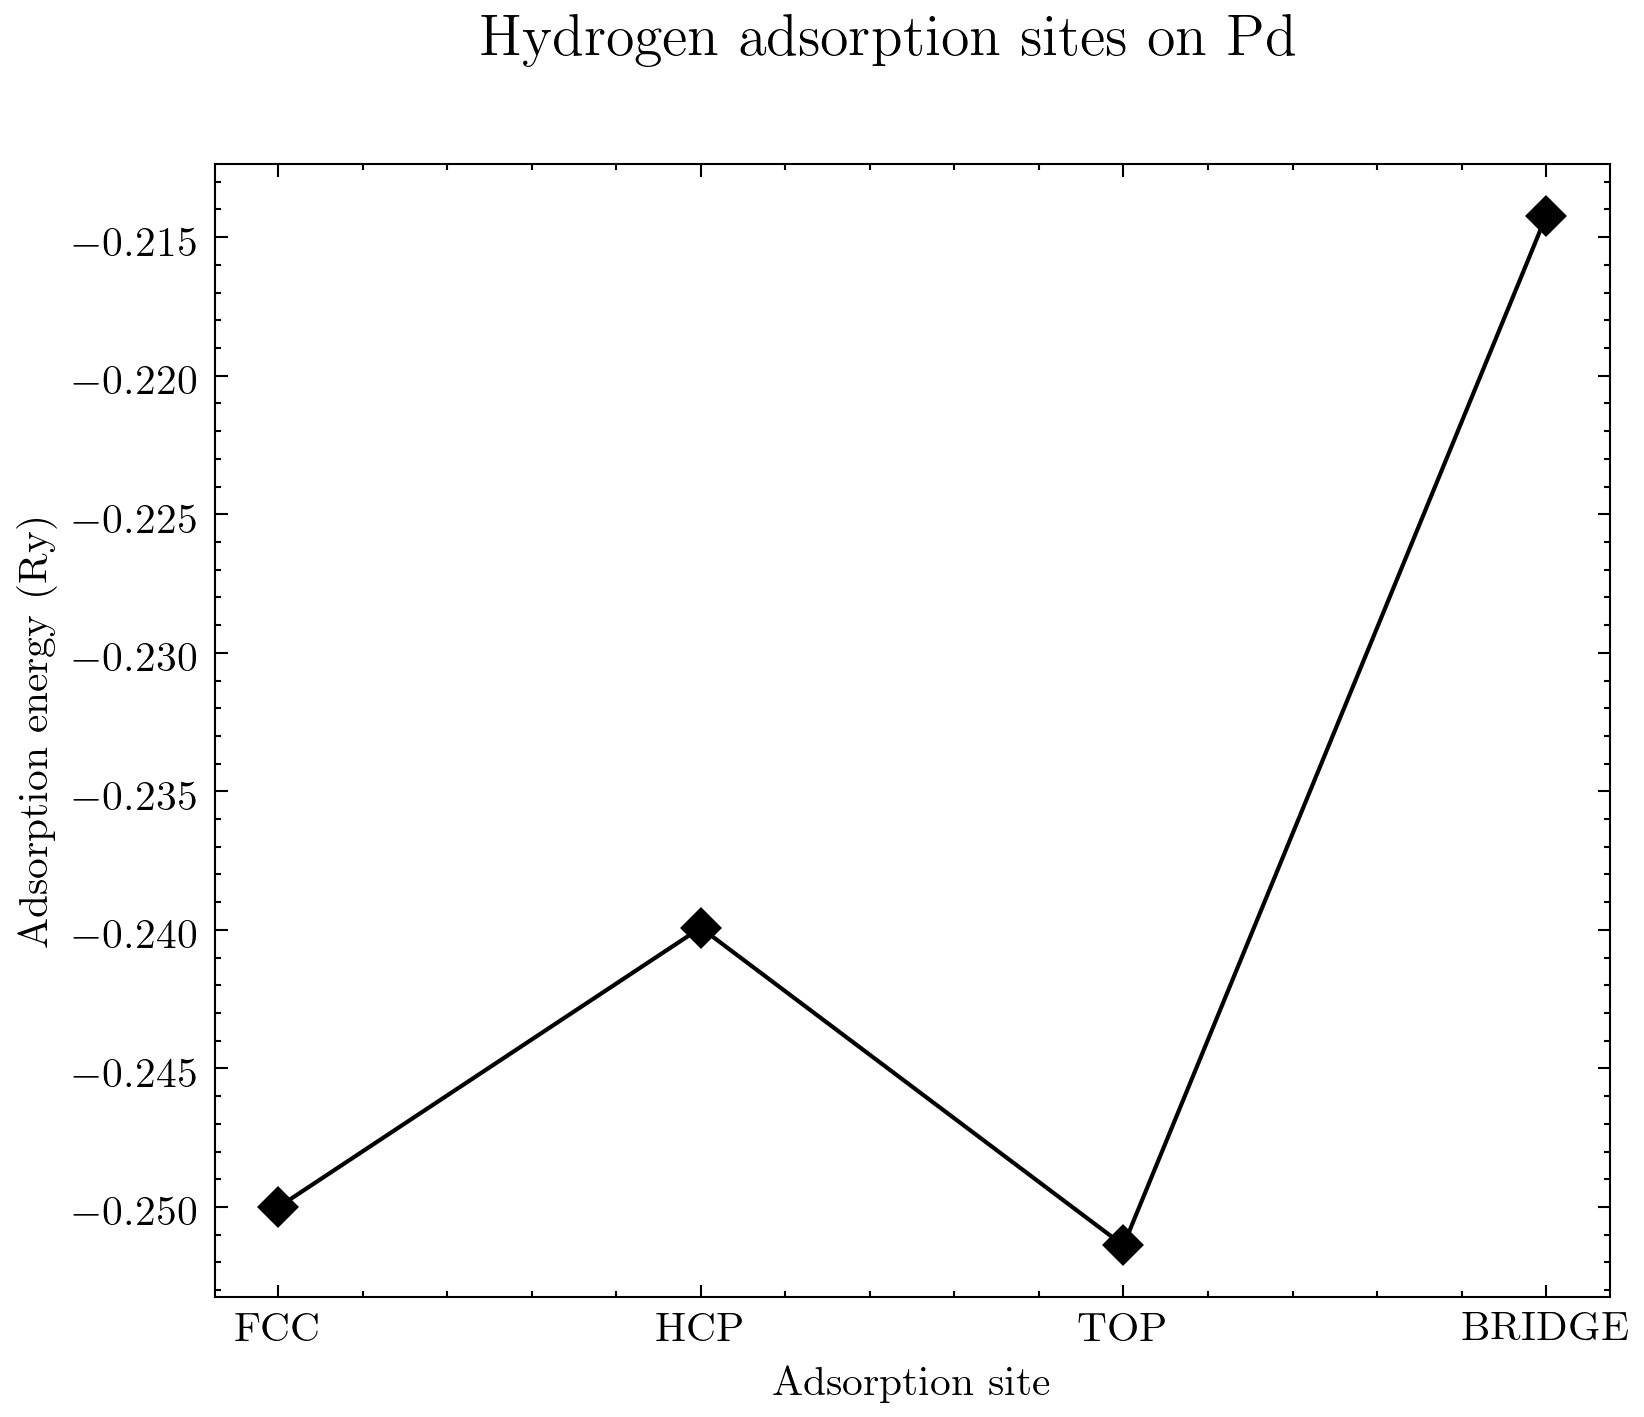
\includegraphics{/Users/marc/Thesis/Chapter3/data/PDSITES.jpg}
  \caption{Adsorption energy of H for each site on a 2x2x5 Pd slab}
  \label{Pdsite}
\end{figure}

Almost all binary alloys show a decreased affinity towards hydrogen adsoprtoion. This is due to hydrogen adsorption energies being closely related to the catalytic activity for hydrogen dissociation of the individual metal elements. The effect appears to be less prevalent for binary alloys with elements with a larger atomic size such as silver which is likely due to the larger atomic size creating a larger area for hydrogen to adsorb within fcc site of the crystalline lattice, which is one of the preferential sites for H adsorption. Zr and Au do not follow this trend however which indicates that the catalytic activity is effected more by electronic interactions than surface geometry. In all cases reduction in palladium from the surface results in lower catalytic activity for hydrogen adsorption which is also likely to be due to the average reduction in number of top sites avaliable for adsorption, which other than fcc is one of the preferential adsorption sites. 

All ternary alloys similarly showed lower catalytic activity than both Pd, and all binary alloys. This again shows that lowering the concentration of Pd in the surface of a membrane has the overall effect of lowering it's catalytic activity for hydrogen adsorption and dissociation with the exception of copper. The ternary alloys with the highest catalytic activity were PdAuAg and PdCuAg which previous experimental results showing that these alloys have higher permeability than other ternary alloys. All Zr containing alloys had lower catalytic activity showing that for hydrogen permeation Zr has the greatest inhibiting effect. The detrimental effects of Zr to the catalytic activity can be lessened by the addition of Au, Ag, or Cu however all are still lower than binary alloys. 

The correlation coefficient for the presence of each metal and it's effect on the resulting adsorption energy was calculated and is shown in table \ref{corrH}. It shows that the resulting inhibiting effect of each element follows the order Ag$<$Cu$<$Au$<$Zr. 

This value is an important benchmark for the following tests and will be compared to the resulting adsorption energies for other impurities. If these impurities show a lower adsorption energy value when compared to hydrogen then they will be preferntially adsorbed and less suitable for use for that type of impurity. It also reveals that the composition of the membrane can largely effect the catalytic activity for dissociation of hydrogen in itself. As membranes become thinner this will result in a shift of the limiting step to catalytic activity and therefore this value must also be optimised to ensure the highest flux can be achieved, however such work is outside the scope of this study. 

\begin{table}[]
  \centering
  \caption{Correlation coefficient of Ag, Au, Cu, Zr addition to Pd with adsorption energy of H}
  \label{corrH}
  \begin{tabular}{@{}cc@{}}
  \toprule
  Metal & Correlation coefficient \\ \midrule
  Ag    & -0.024666               \\
  Au    & 0.259205                \\
  Cu    & 0.019221                \\
  Zr    & 0.347930                \\ \bottomrule
  \end{tabular}
  \end{table}




\begin{landscape}
\begin{figure}
    \centering
    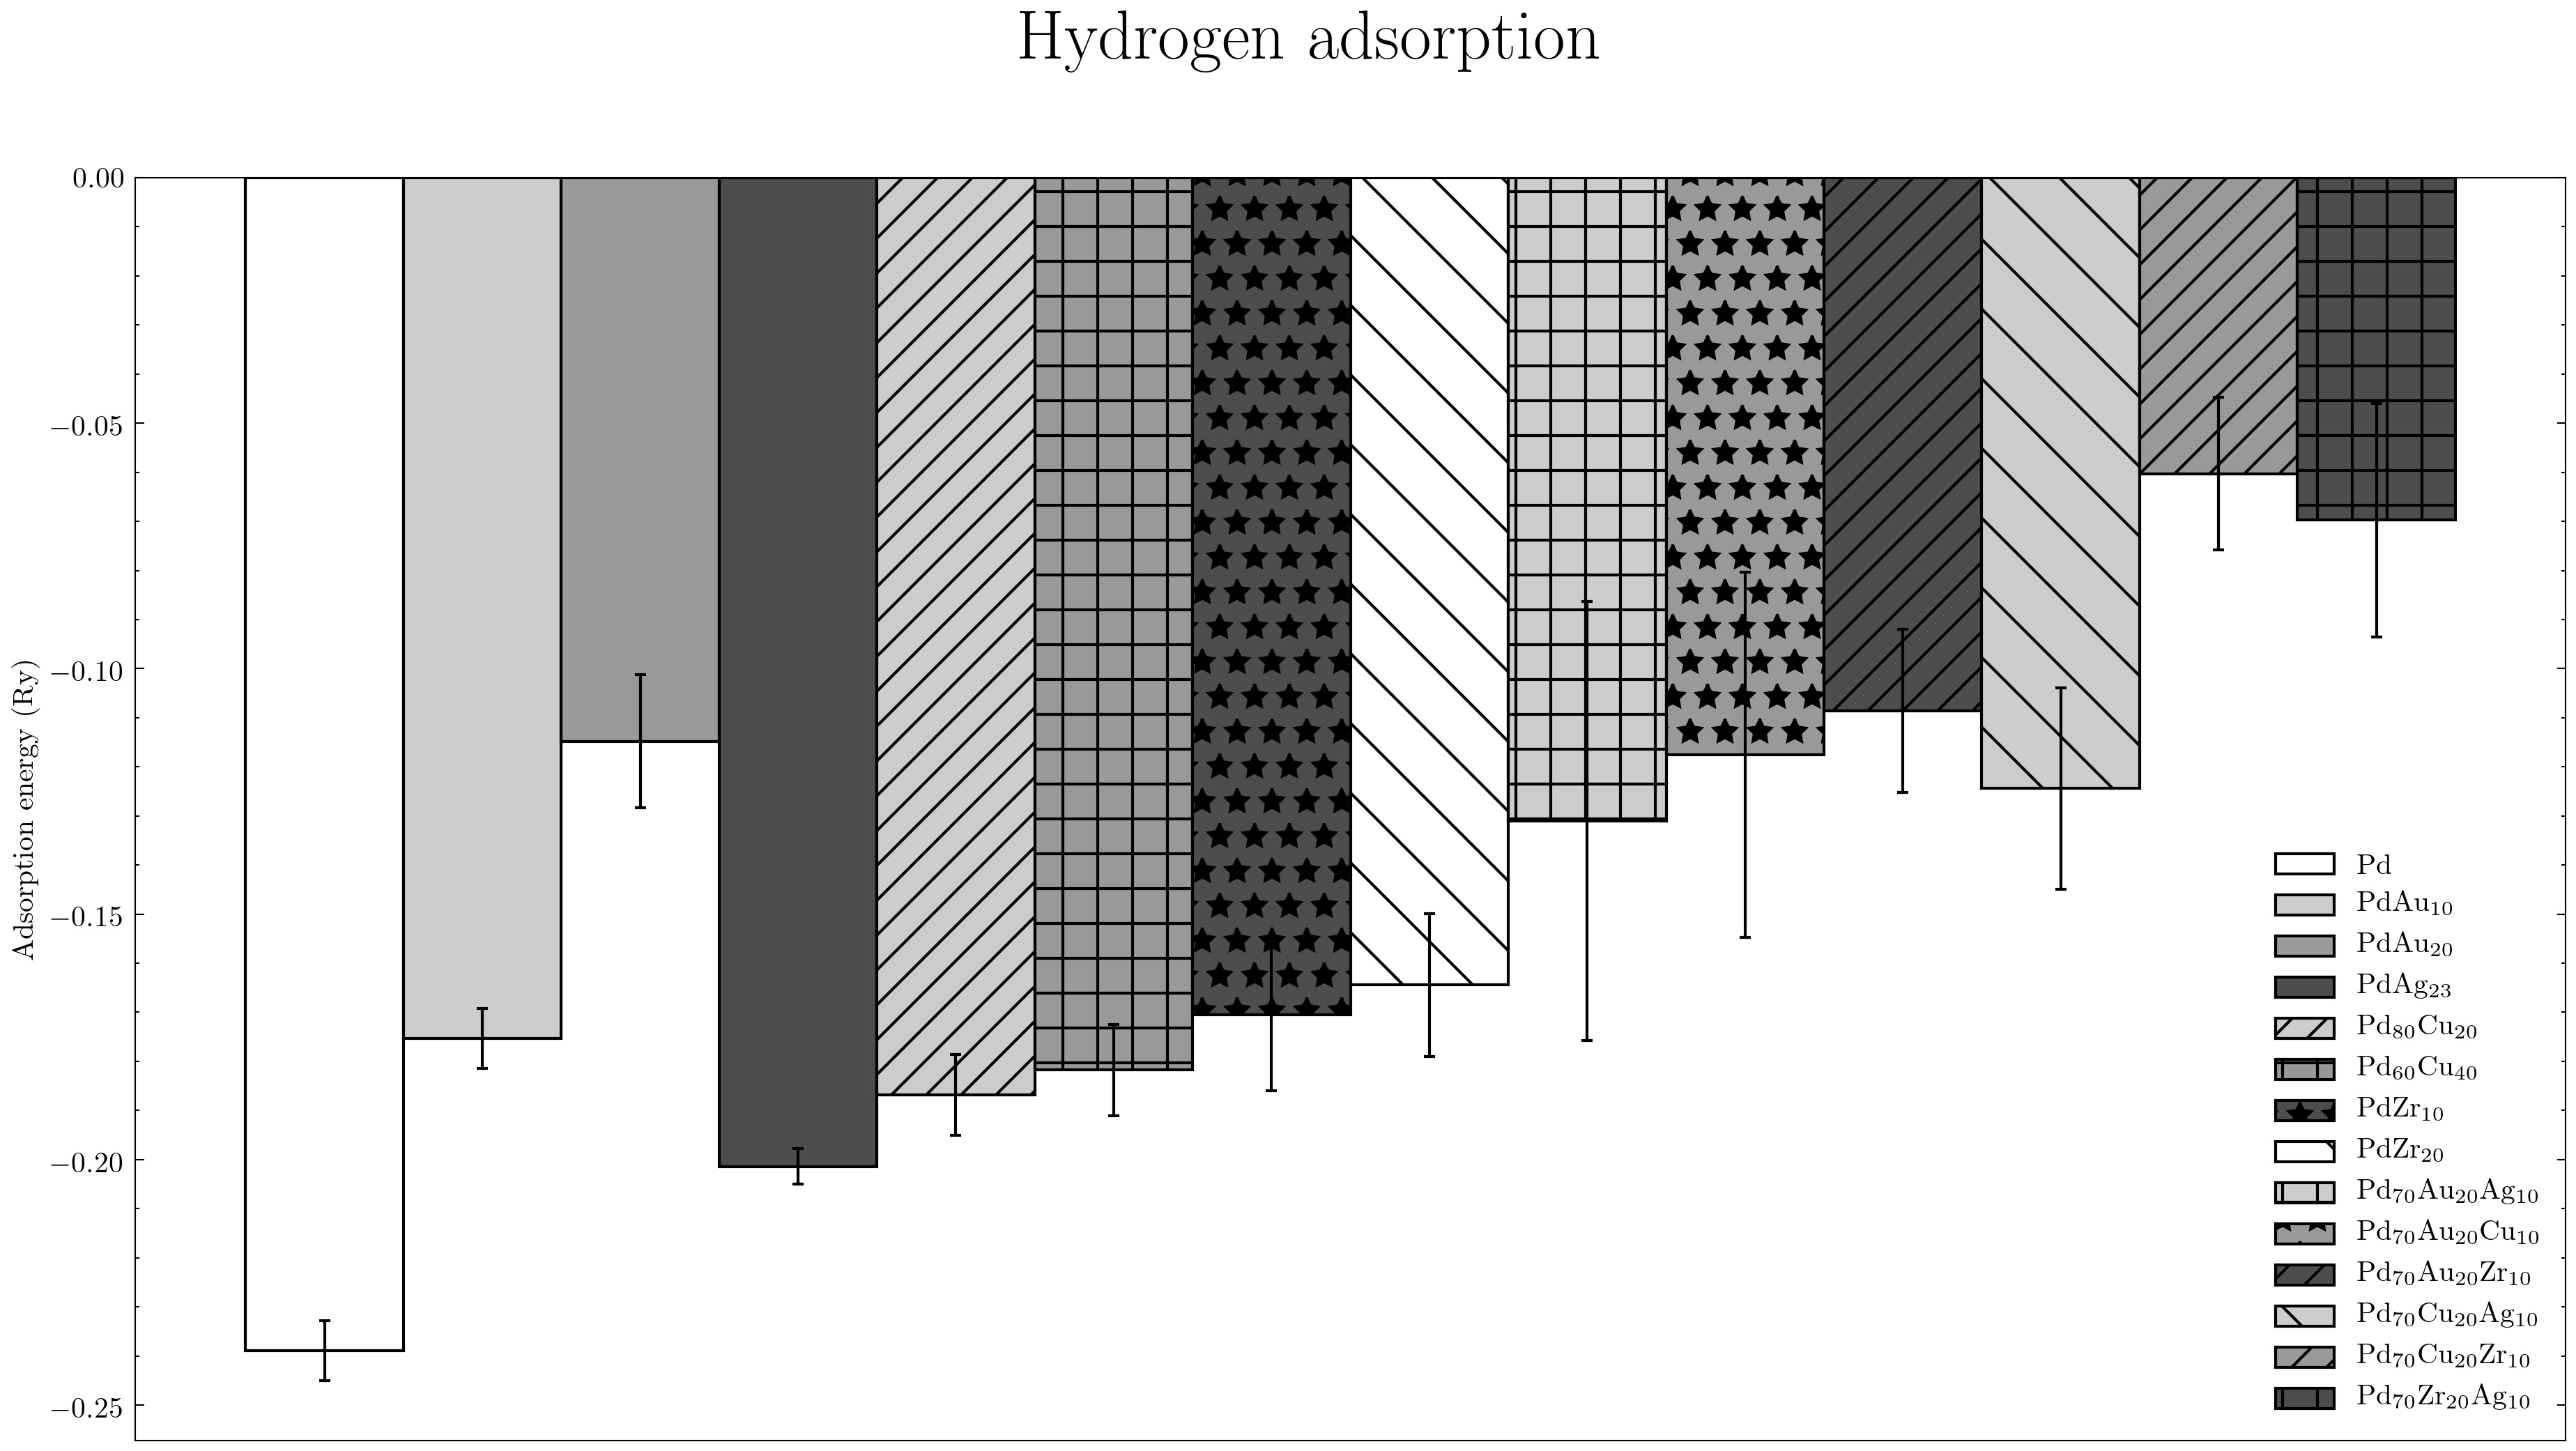
\includegraphics[width=0.9\linewidth,height=\textheight, keepaspectratio]{/Users/marc/Thesis/Chapter3/data/h2ads.jpg}
    \caption{Average adsorption energy of H\textsubscript{2} on the surface of palladium and palladium alloy slabs}
    \label{h2ads}
  \end{figure}

\end{landscape}
\subsubsection{Helium, Nitrogen, Carbon Dioxide and Argon}

\begin{landscape}
  \begin{figure}
      \centering
      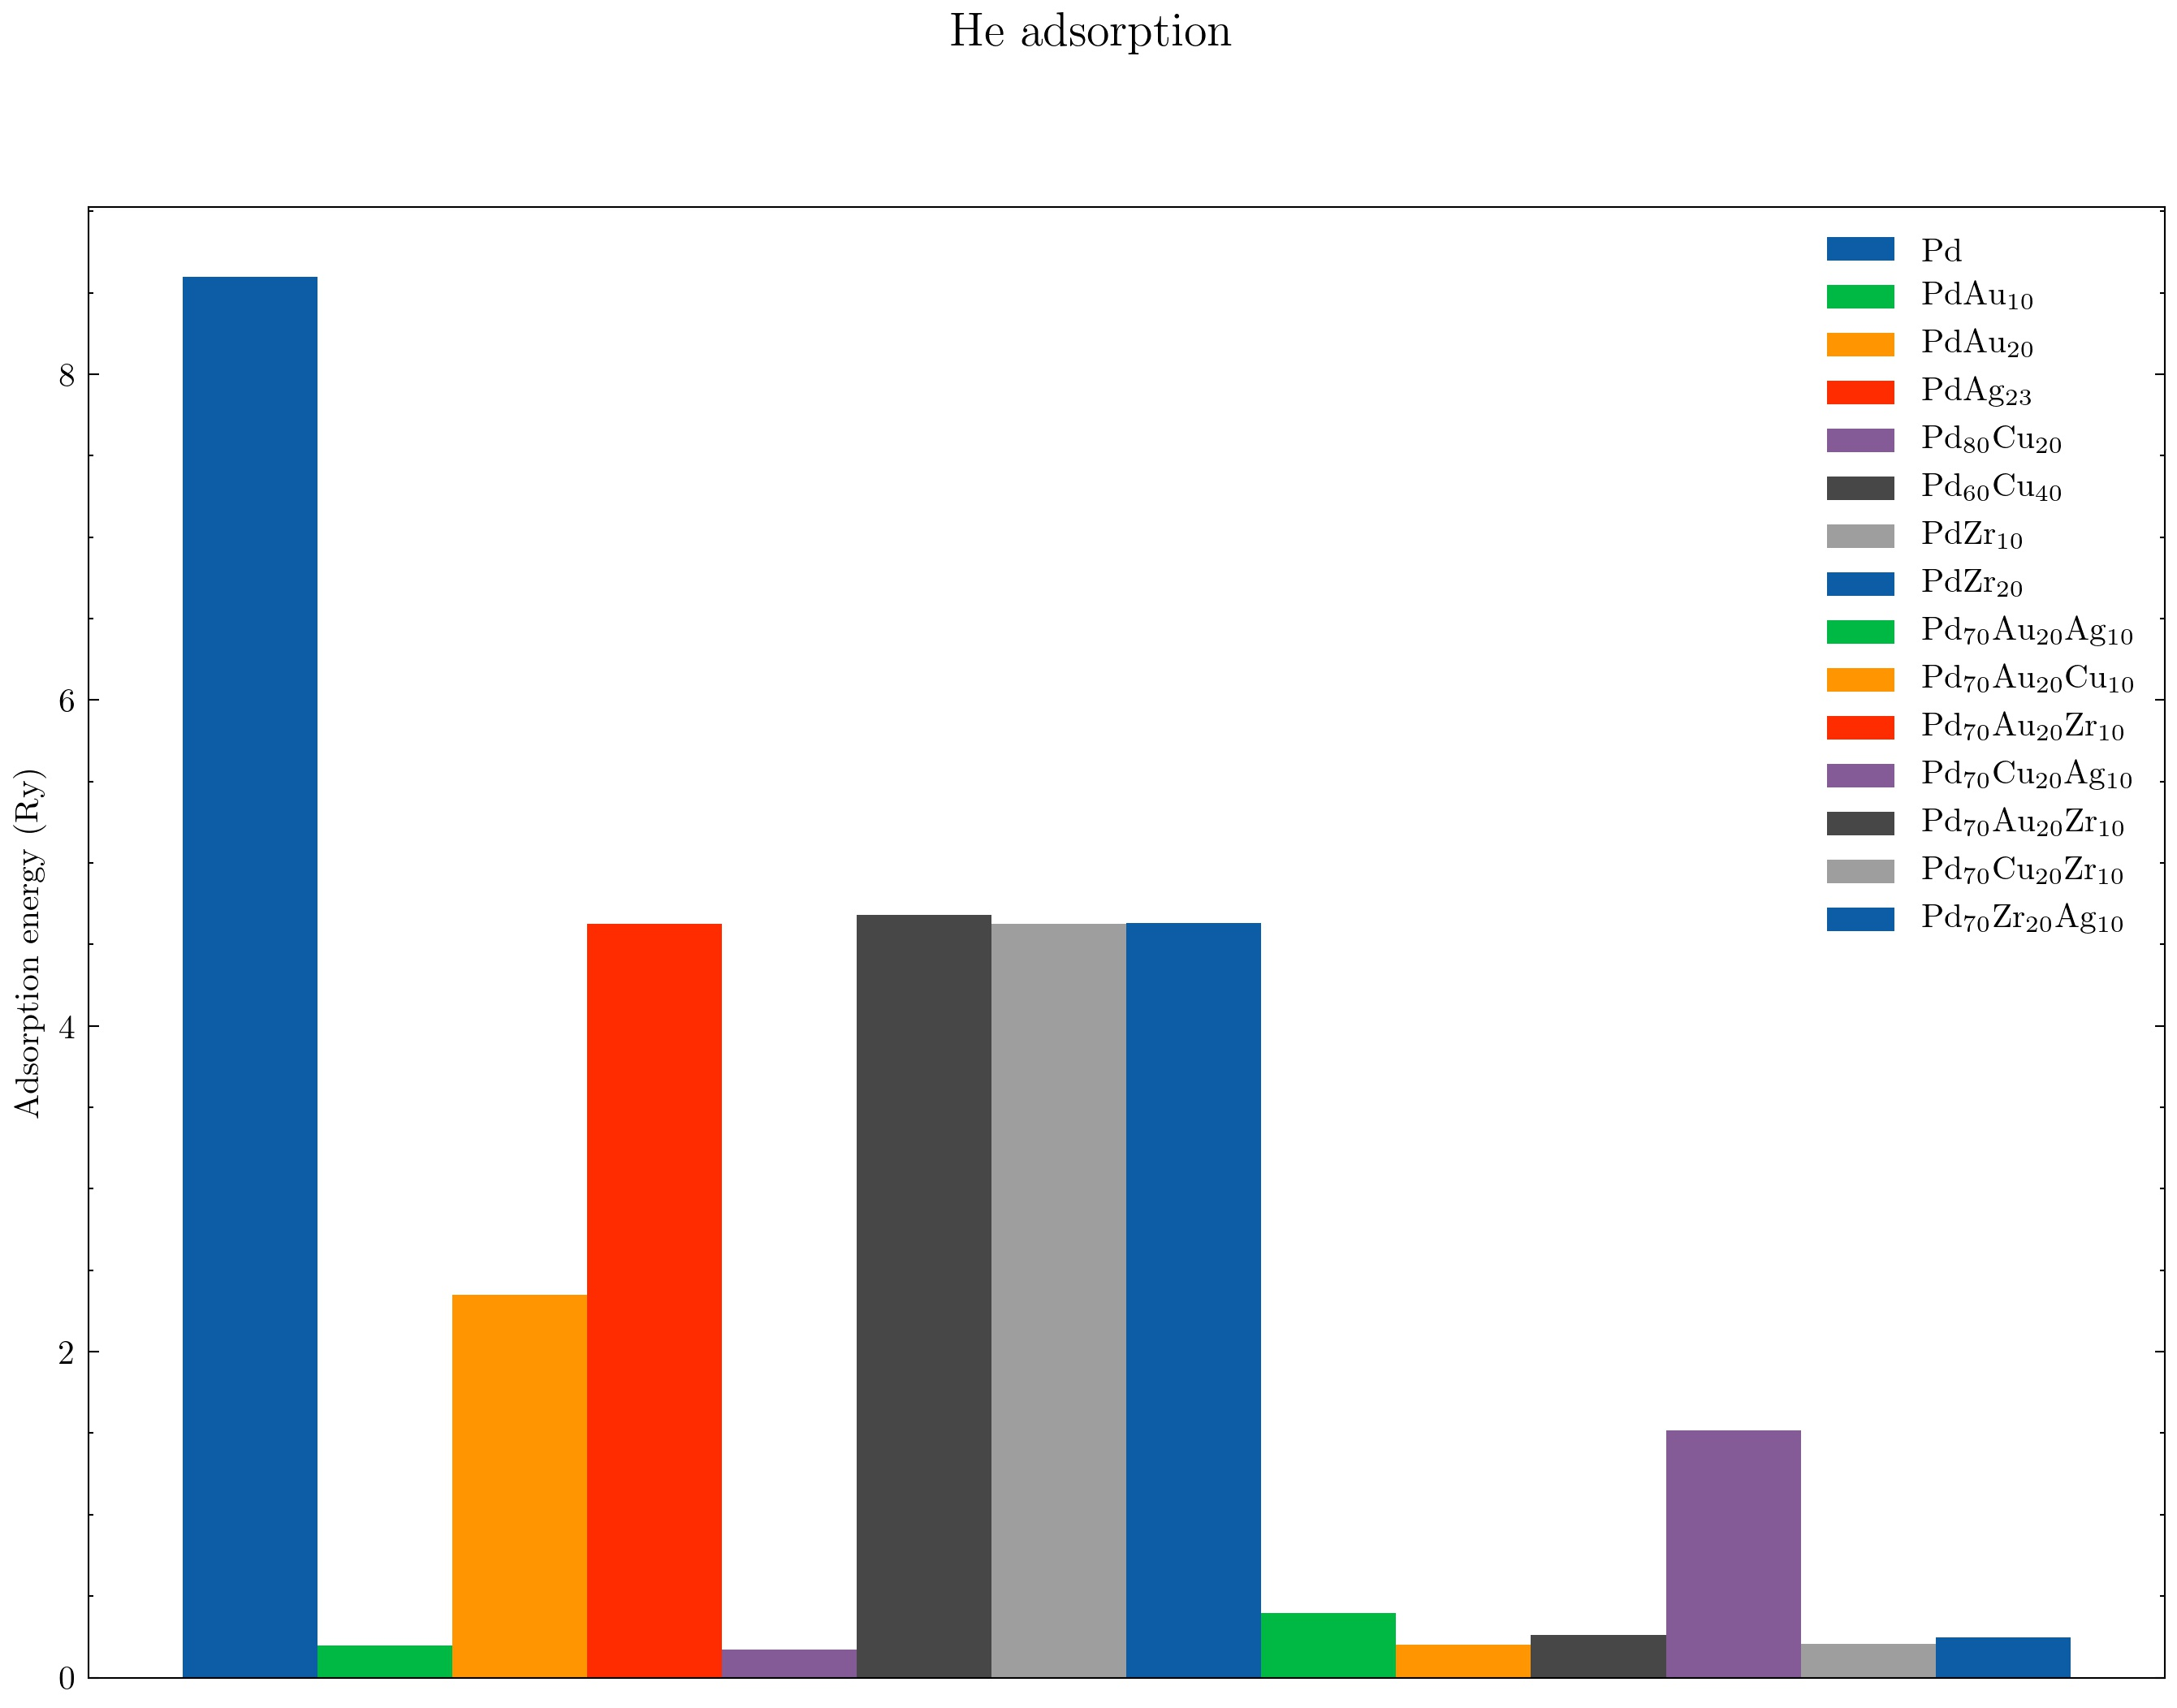
\includegraphics[width=0.9\linewidth,height=\textheight, keepaspectratio]{/Users/marc/Thesis/Chapter3/data/HEads.jpg}
      \caption{Average adsorption energy of He on the surface of palladium and palladium alloy slabs}
      \label{heads}
    \end{figure}
  
  \end{landscape}

  \begin{landscape}
    \begin{figure}
        \centering
        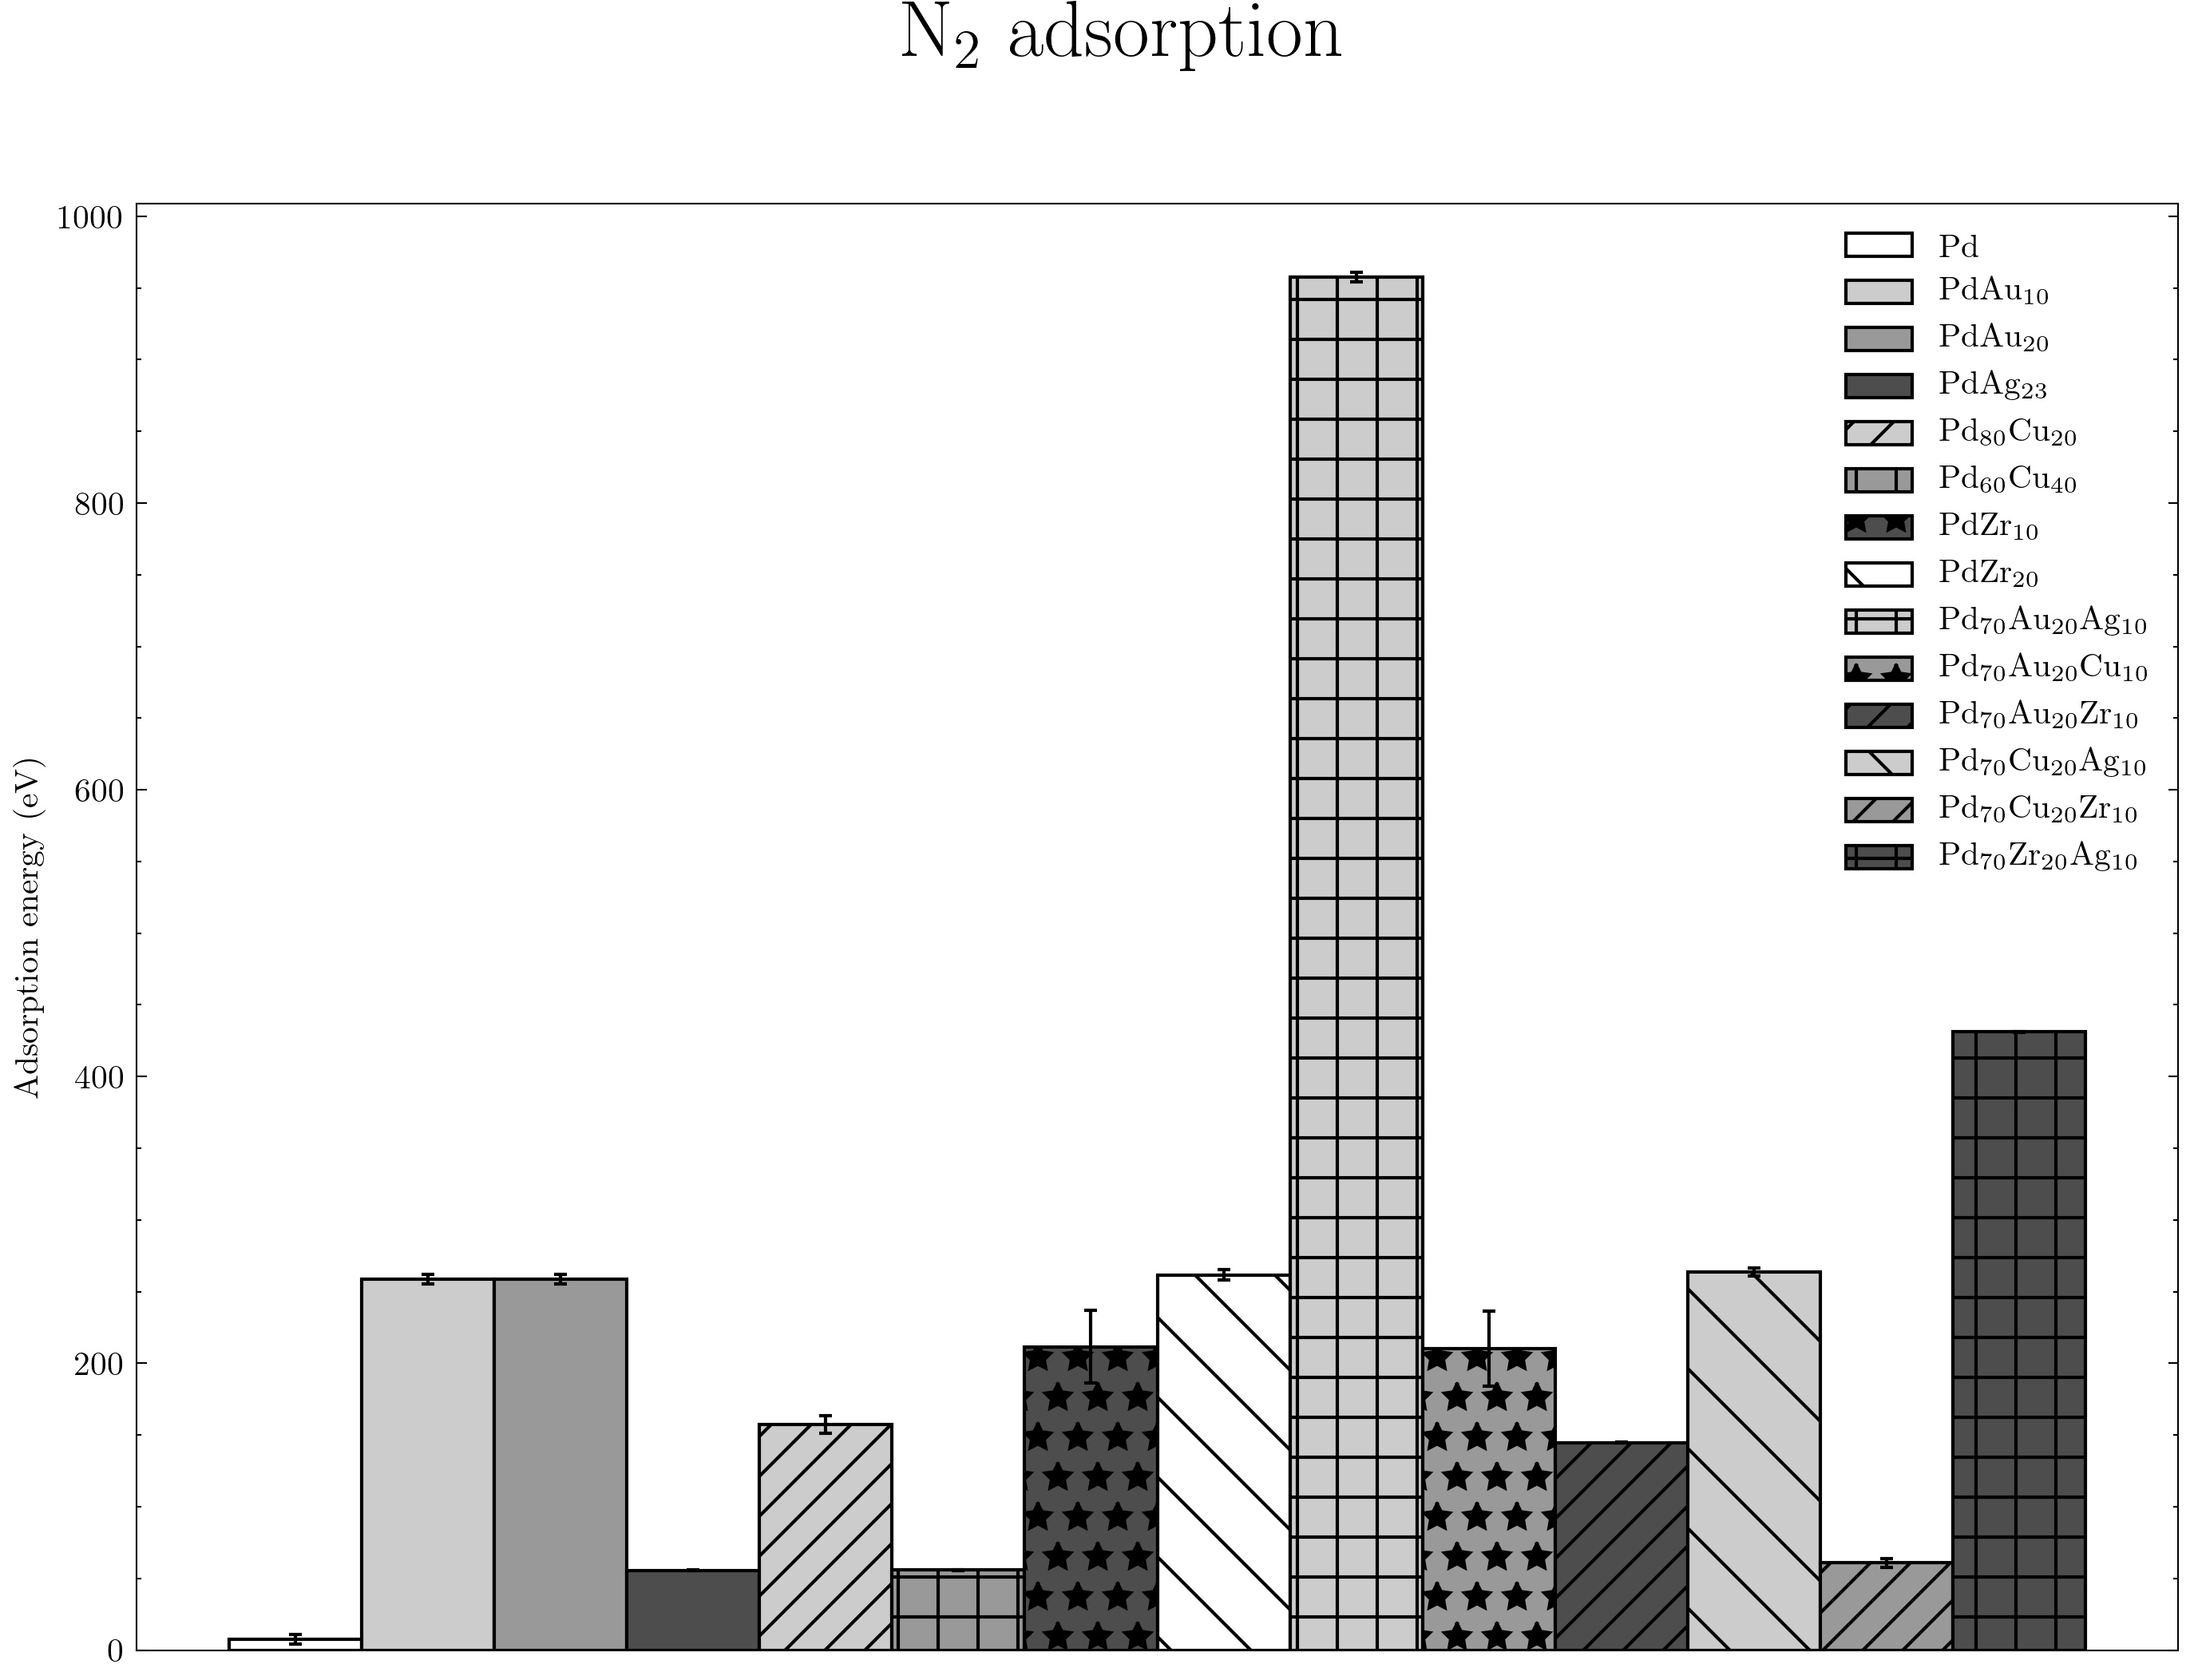
\includegraphics[width=0.9\linewidth,height=\textheight, keepaspectratio]{/Users/marc/Thesis/Chapter3/data/N2ads.jpg}
        \caption{Average adsorption energy of N2 on the surface of palladium and palladium alloy slabs}
        \label{n2ads}
      \end{figure}
    
    \end{landscape}


\begin{landscape}
    \begin{figure}
        \centering
        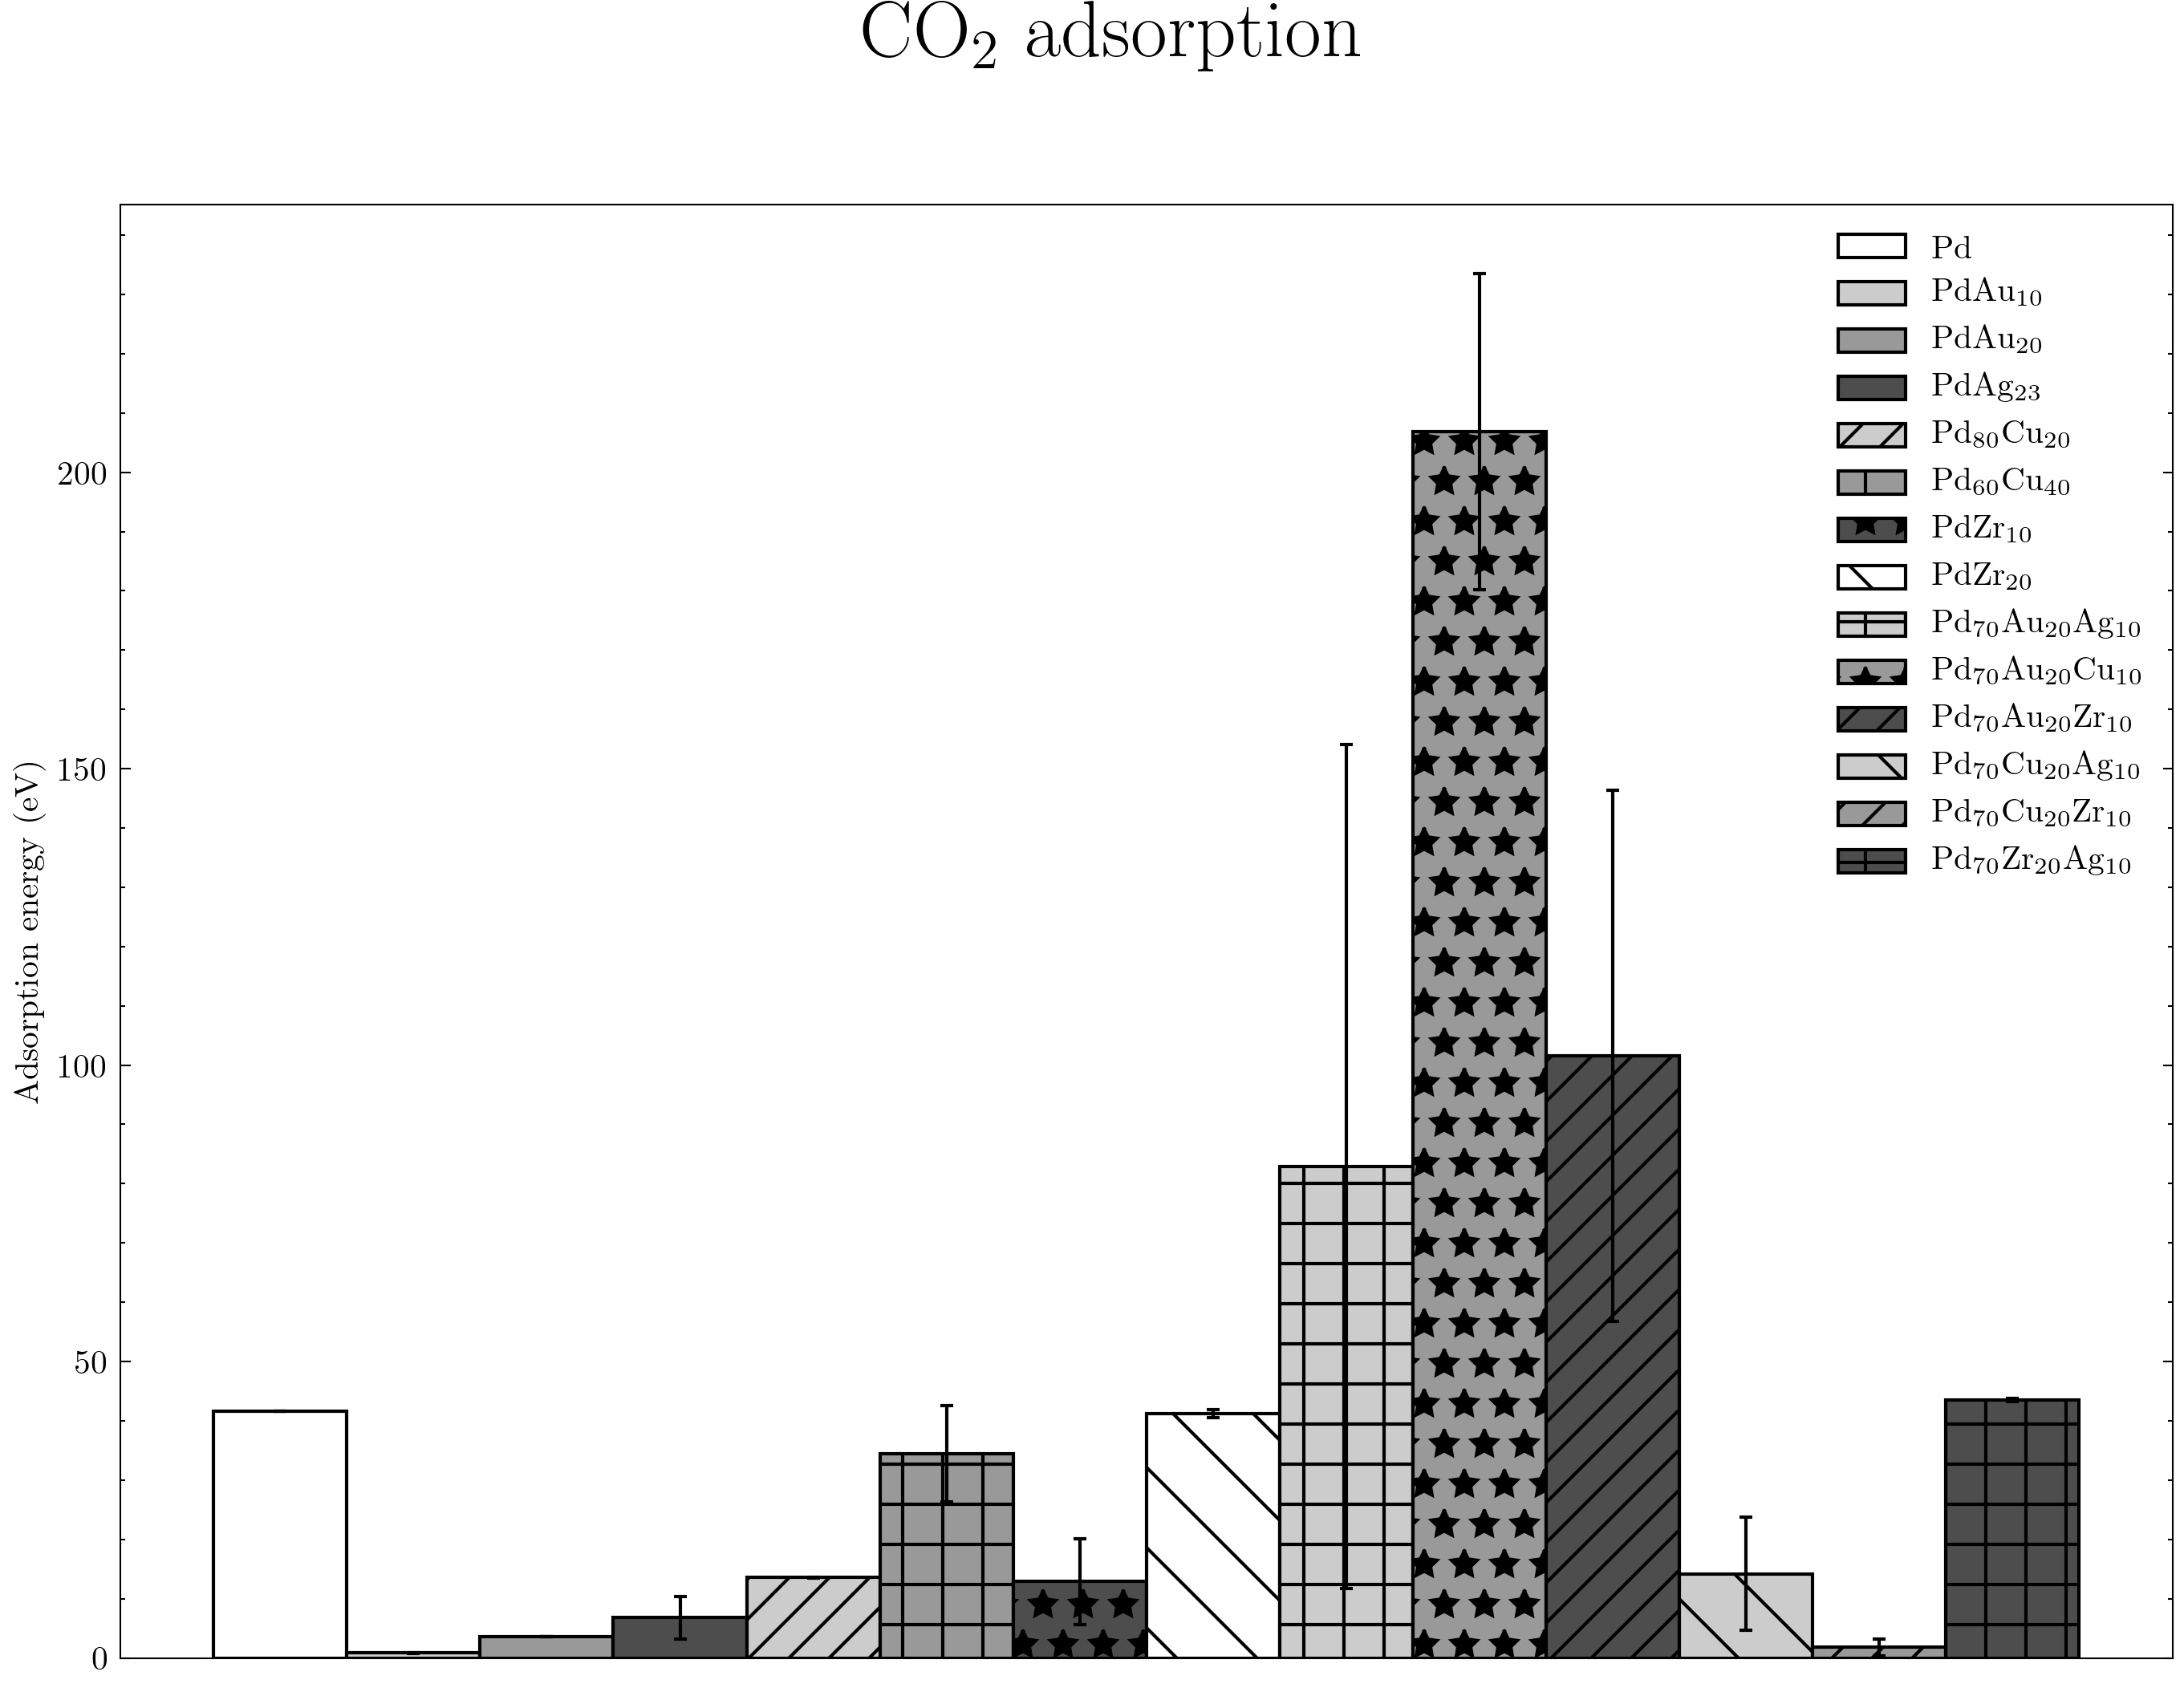
\includegraphics[width=0.9\linewidth,height=\textheight, keepaspectratio]{/Users/marc/Thesis/Chapter3/data/CO2ads.jpg}
        \caption{Average adsorption energy of CO\textsubscript{2} on the surface of palladium and palladium alloy slabs}
        \label{co2ads}
      \end{figure}
    
    \end{landscape}

    \begin{landscape}
        \begin{figure}
            \centering
            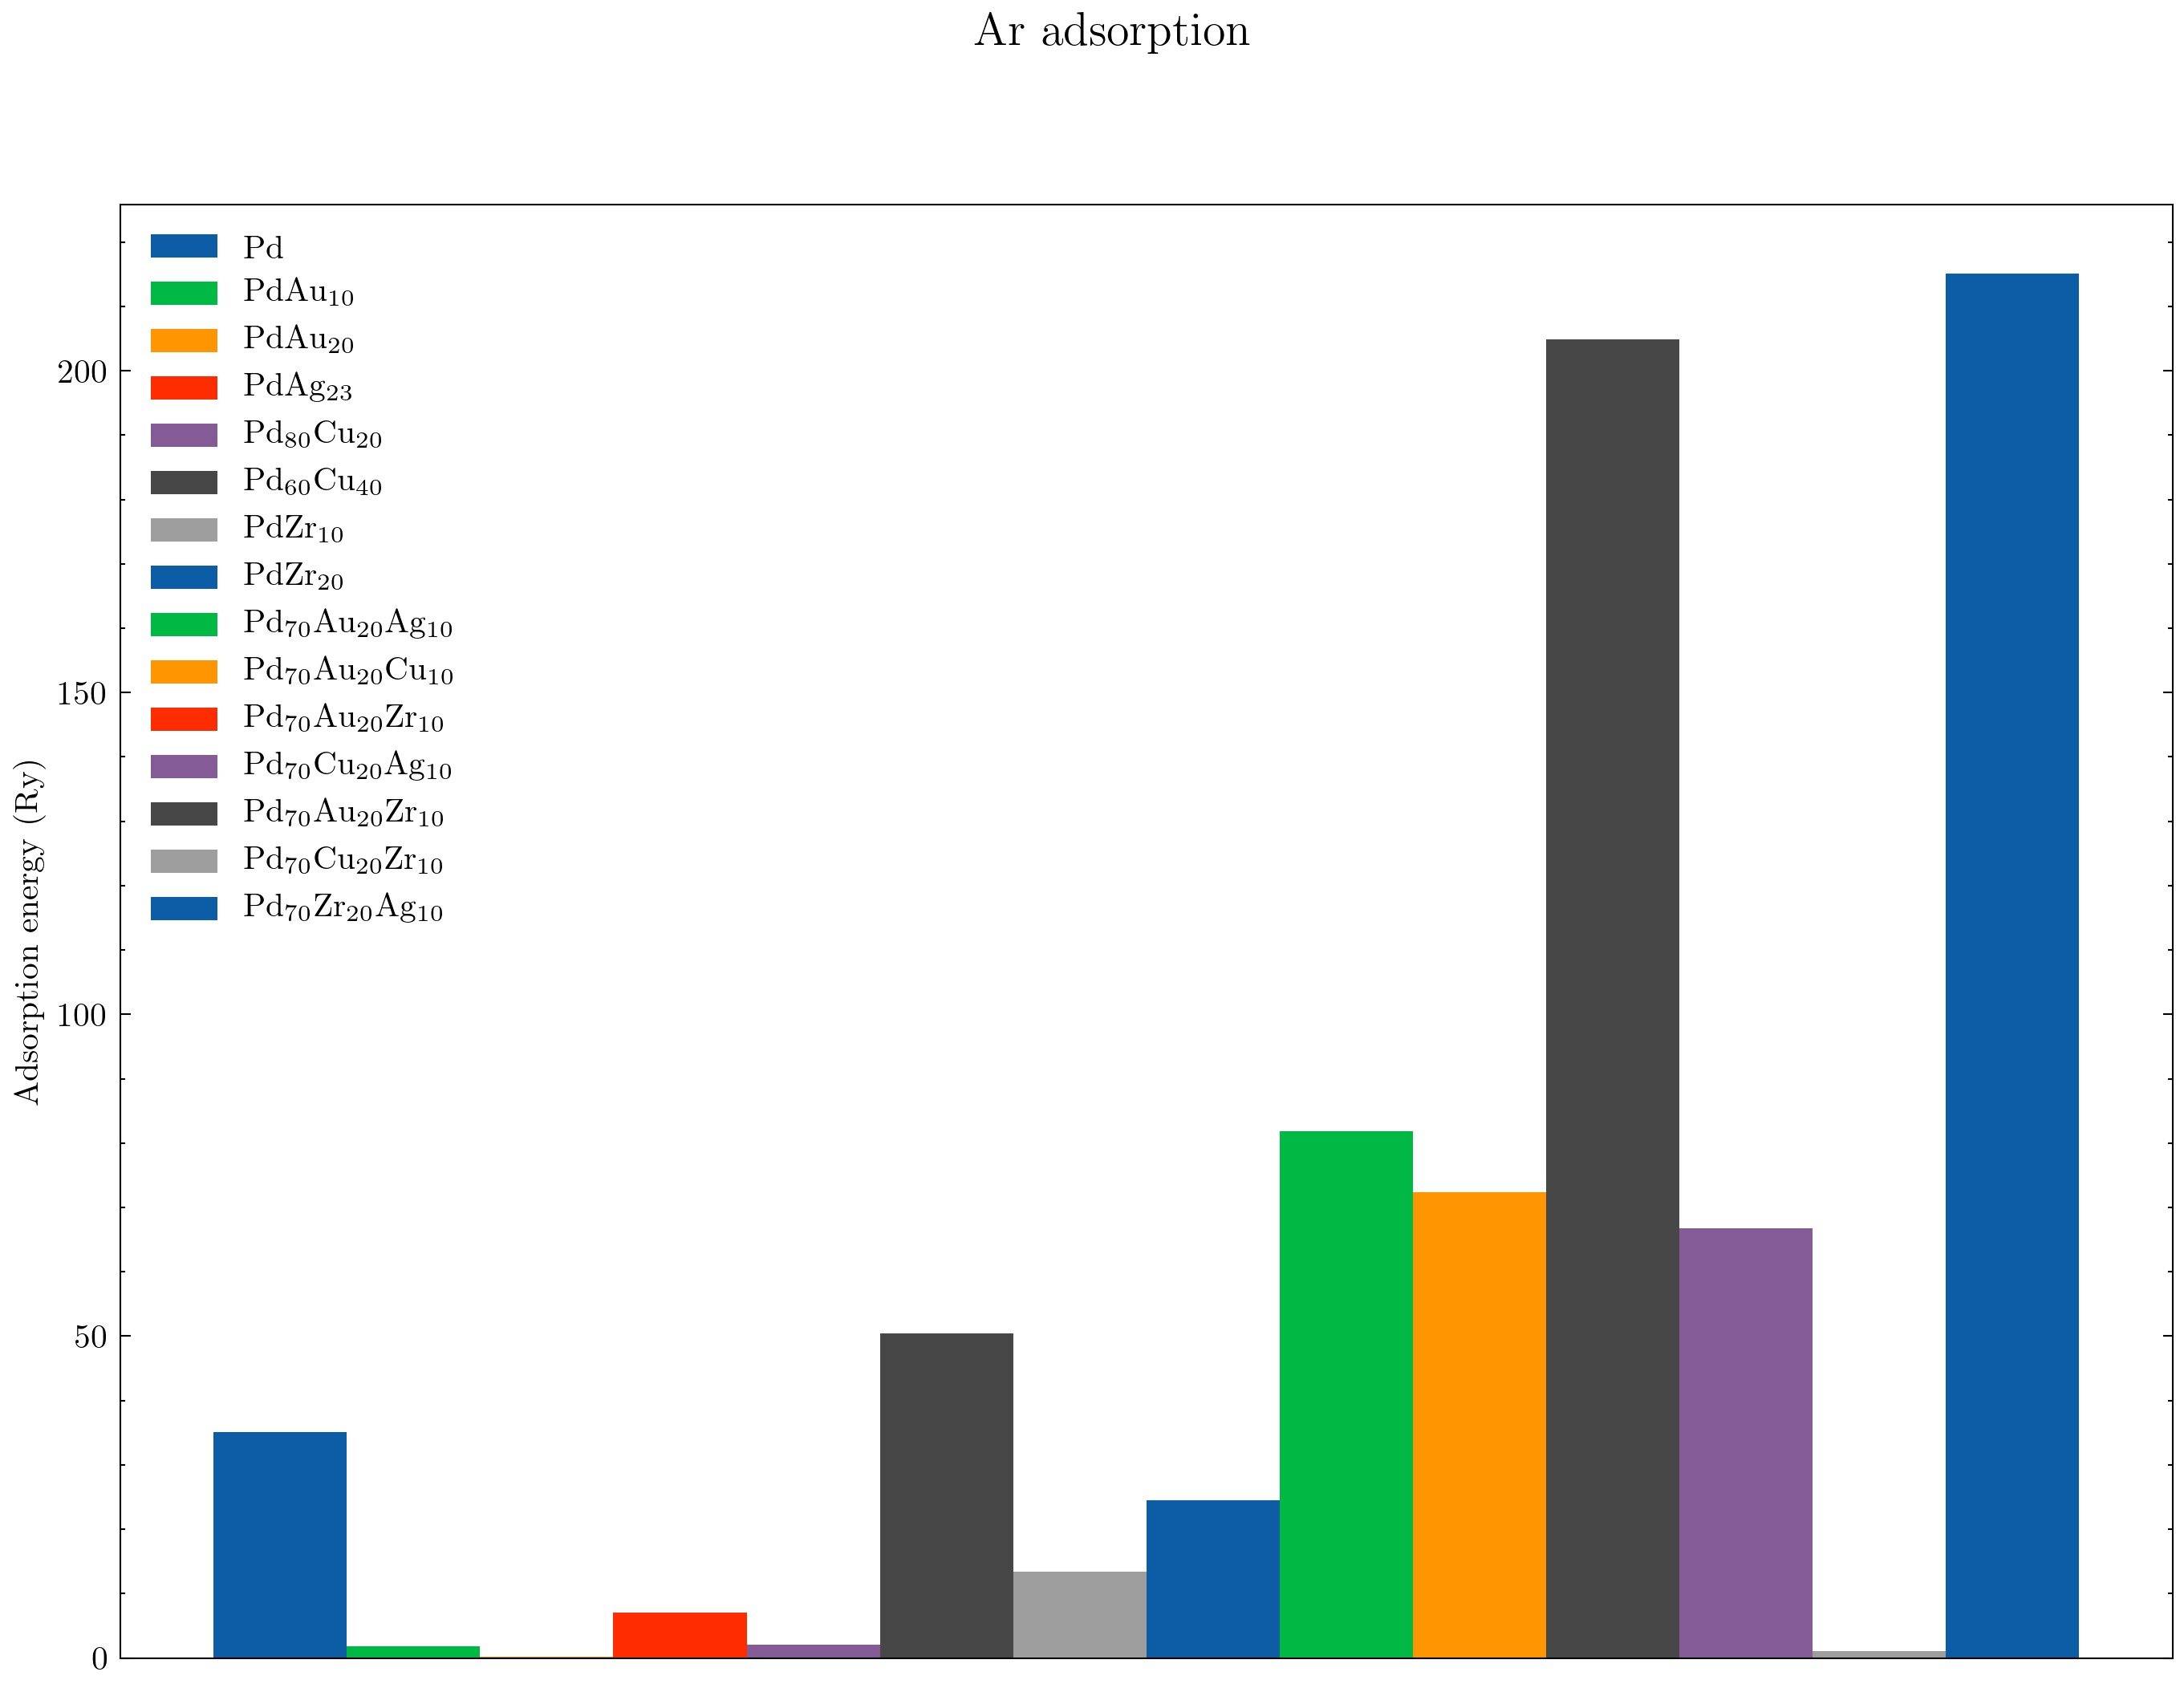
\includegraphics[width=0.9\linewidth,height=\textheight, keepaspectratio]{/Users/marc/Thesis/Chapter3/data/ARads.jpg}
            \caption{Average adsorption energy of Ar on the surface of palladium and palladium alloy slabs}
            \label{Arads}
          \end{figure}
        
        \end{landscape}
\subsubsection{Carbon Monoxide}

\begin{landscape}
    \begin{figure}
        \centering
        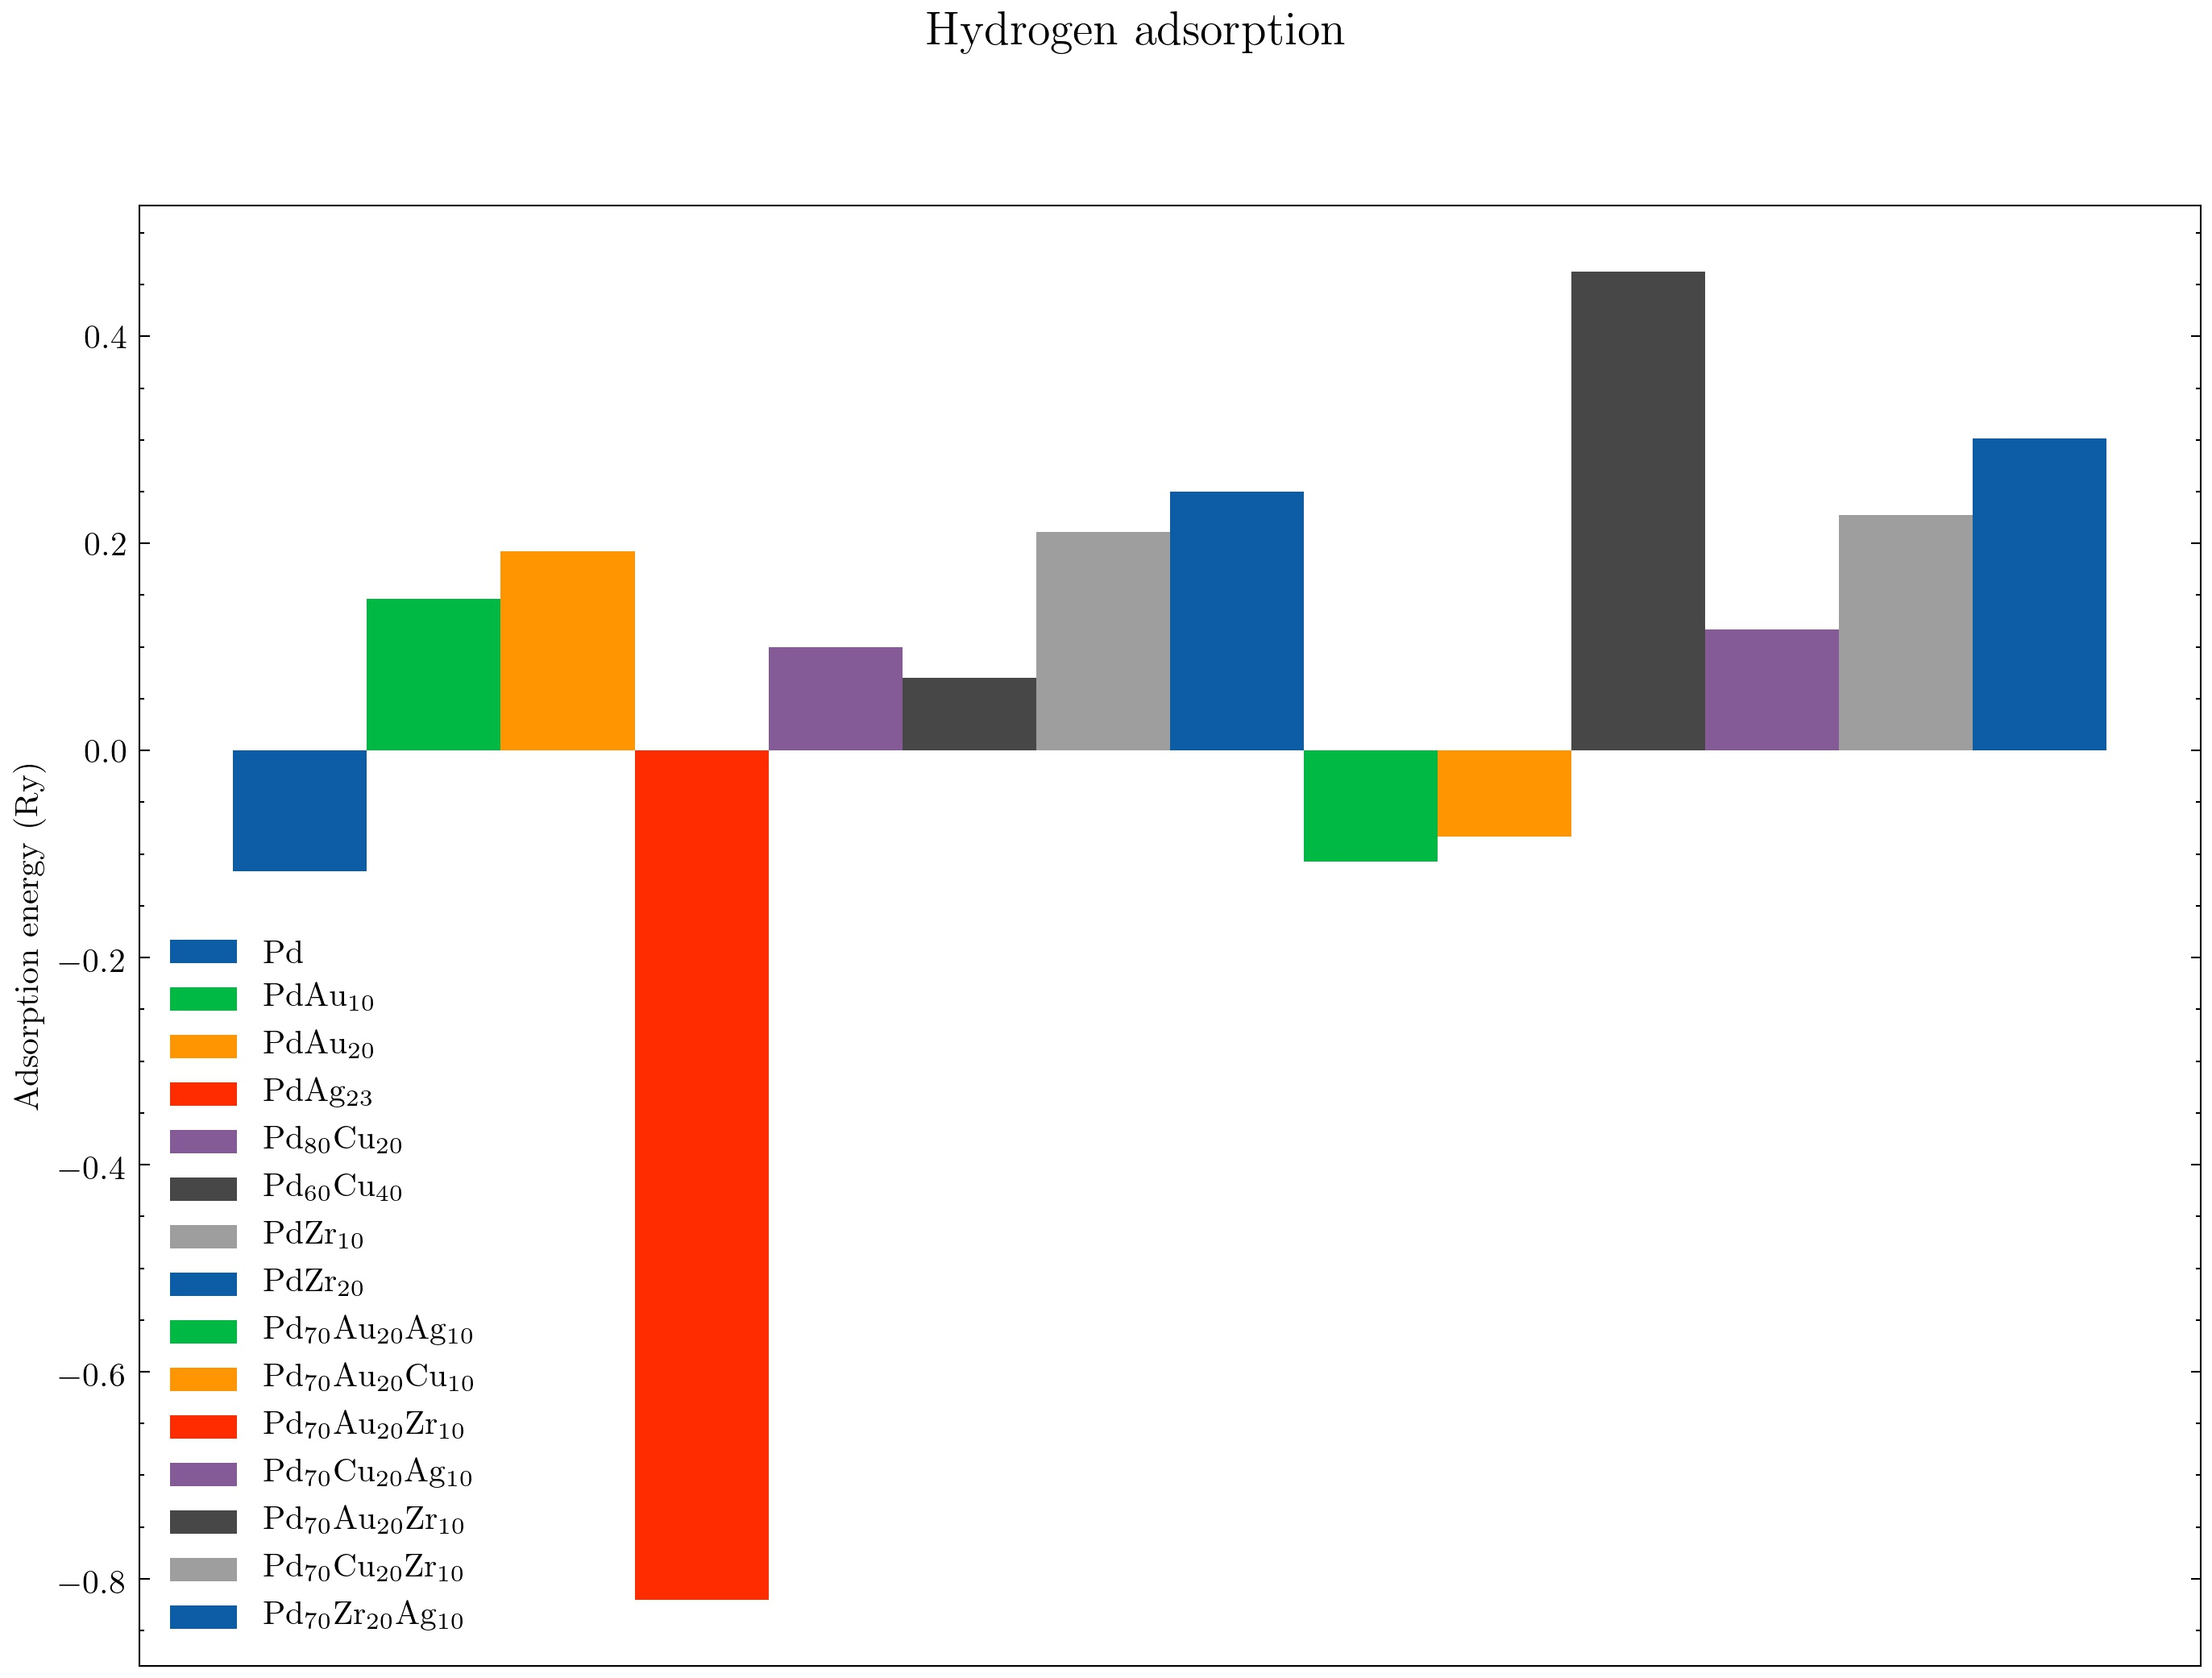
\includegraphics[width=0.9\linewidth,height=\textheight, keepaspectratio]{/Users/marc/Thesis/Chapter3/data/COads.jpg}
        \caption{Average adsorption energy of CO on the surface of palladium and palladium alloy slabs}
        \label{coads}
      \end{figure}
    
    \end{landscape}
\subsubsection{Ammonia}
\begin{landscape}
  \begin{figure}
      \centering
      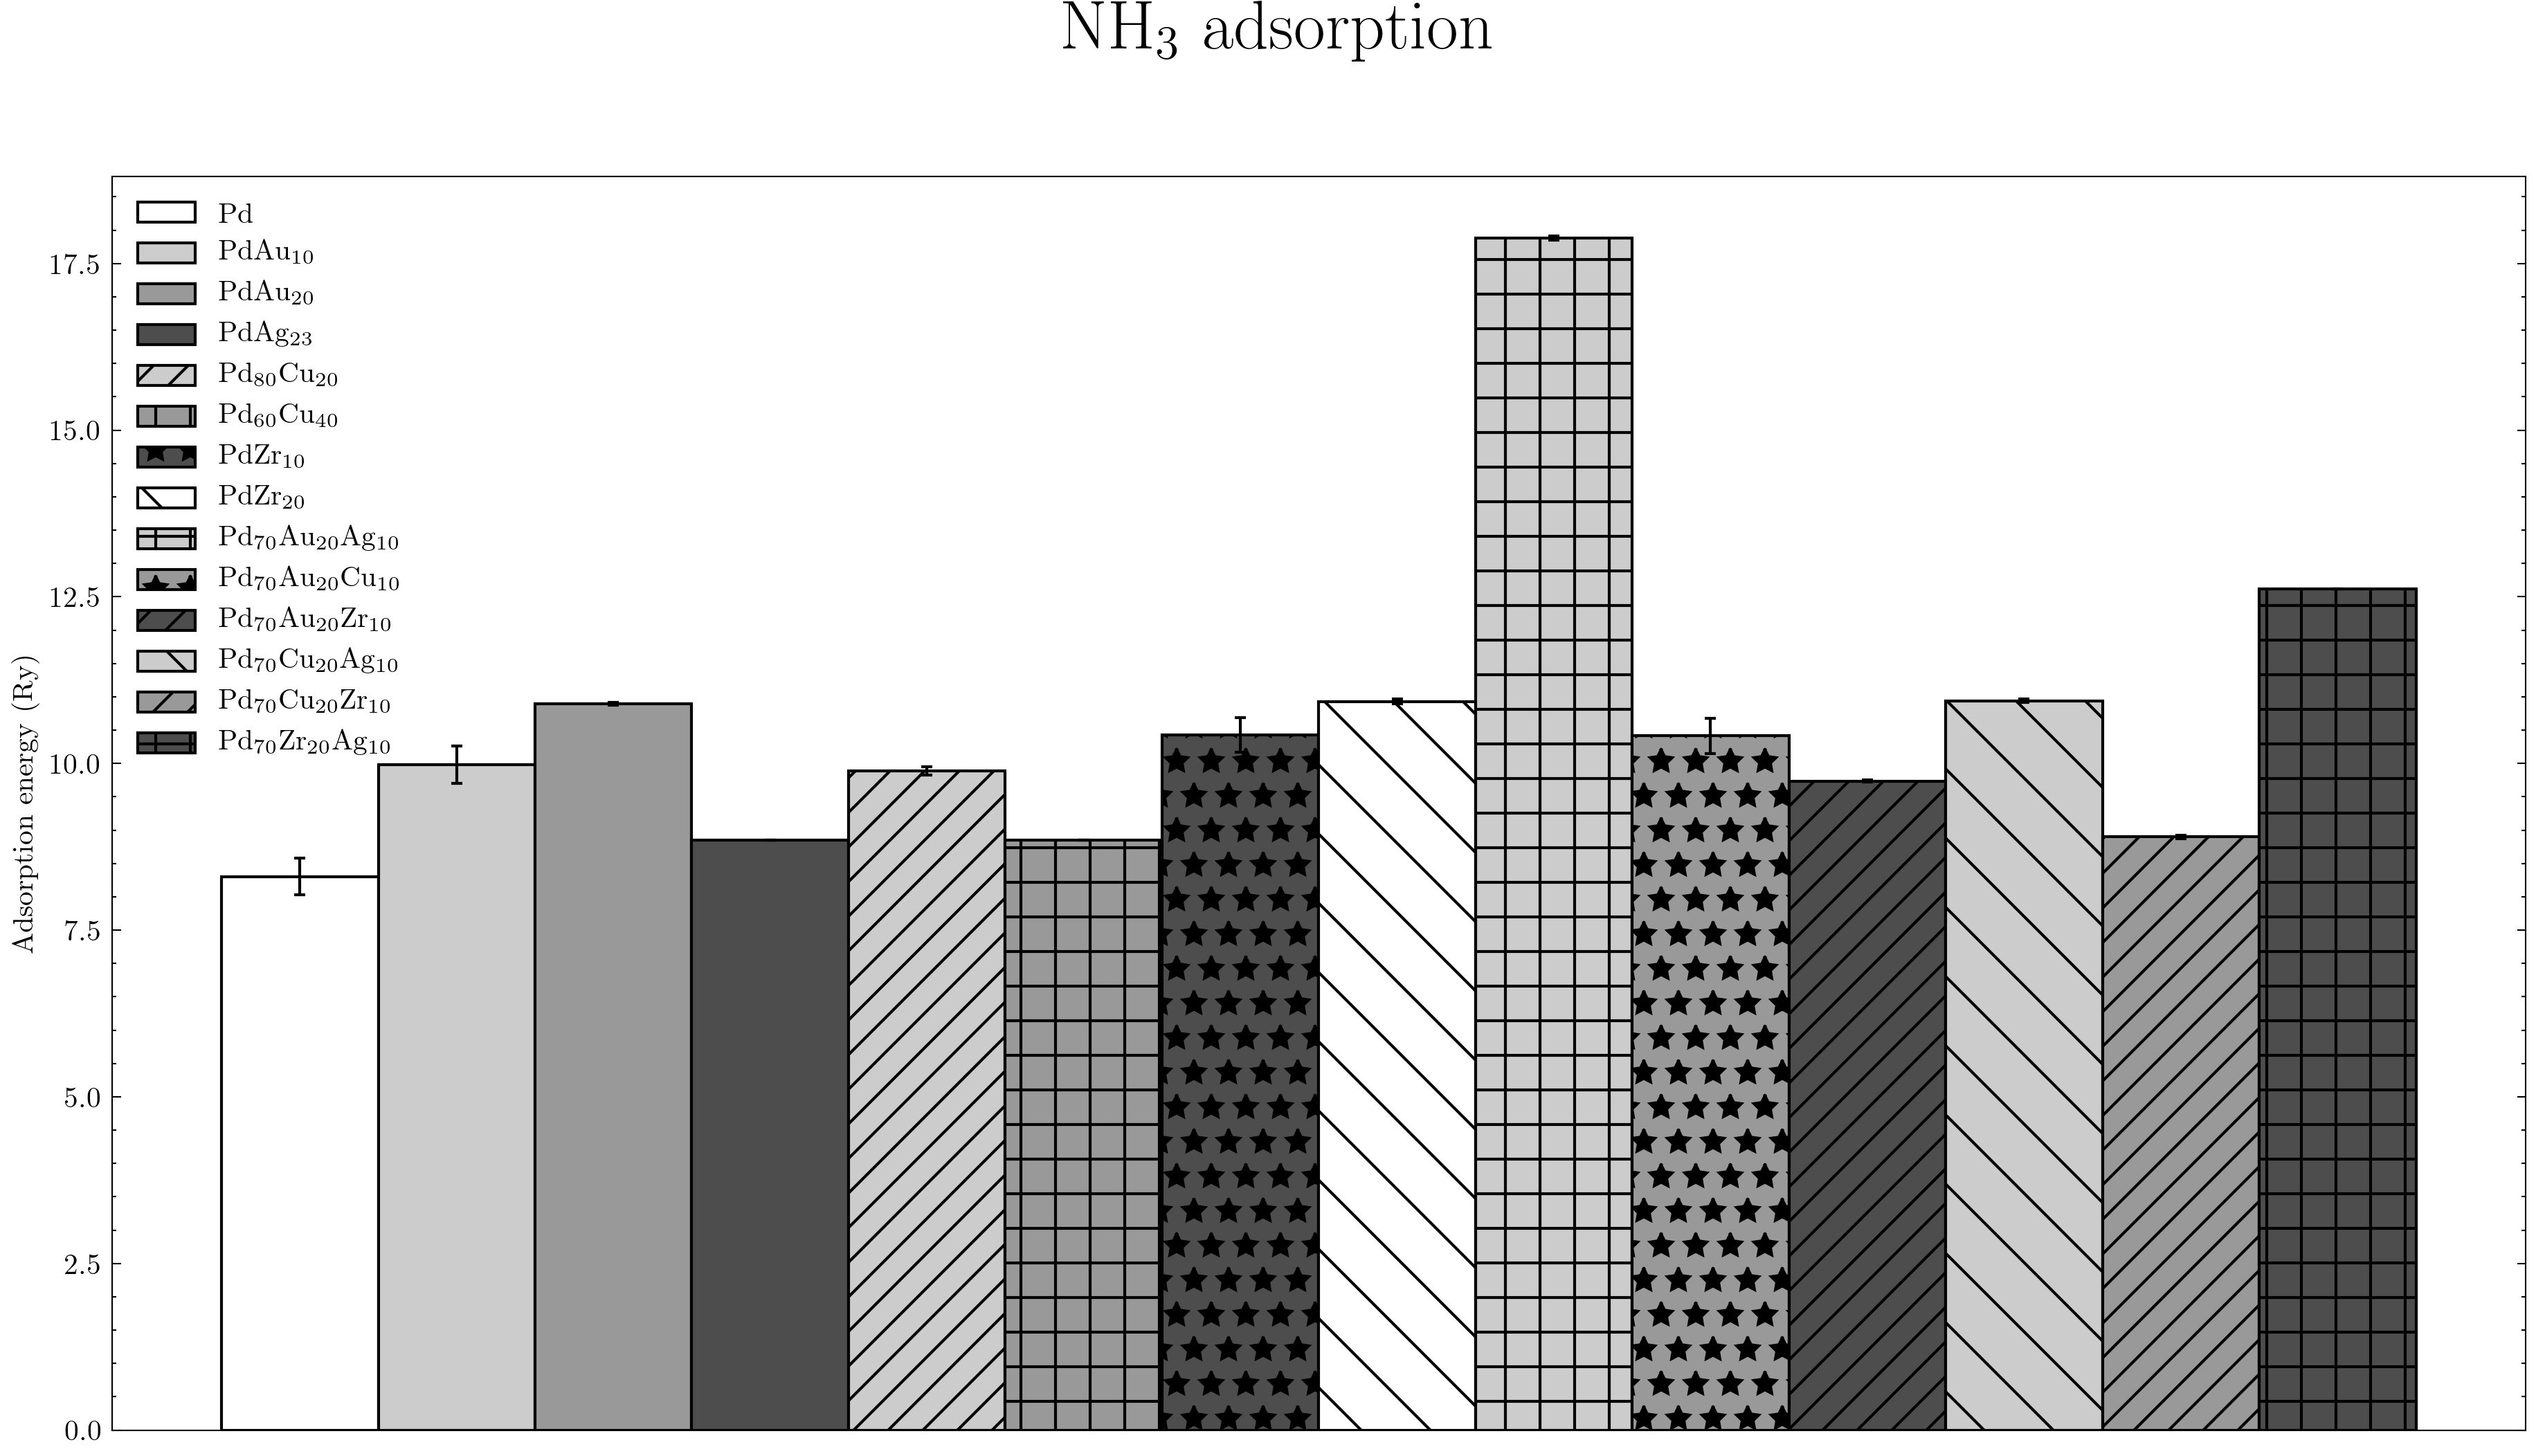
\includegraphics[width=0.9\linewidth,height=\textheight, keepaspectratio]{/Users/marc/Thesis/Chapter3/data/NH3ads.jpg}
      \caption{Average adsorption energy of NH\textsubscript{3} on the surface of palladium and palladium alloy slabs}
      \label{nh3ads}
    \end{figure}
  
  \end{landscape}
\subsubsection{Oxygen}

\begin{landscape}
  \begin{figure}
      \centering
      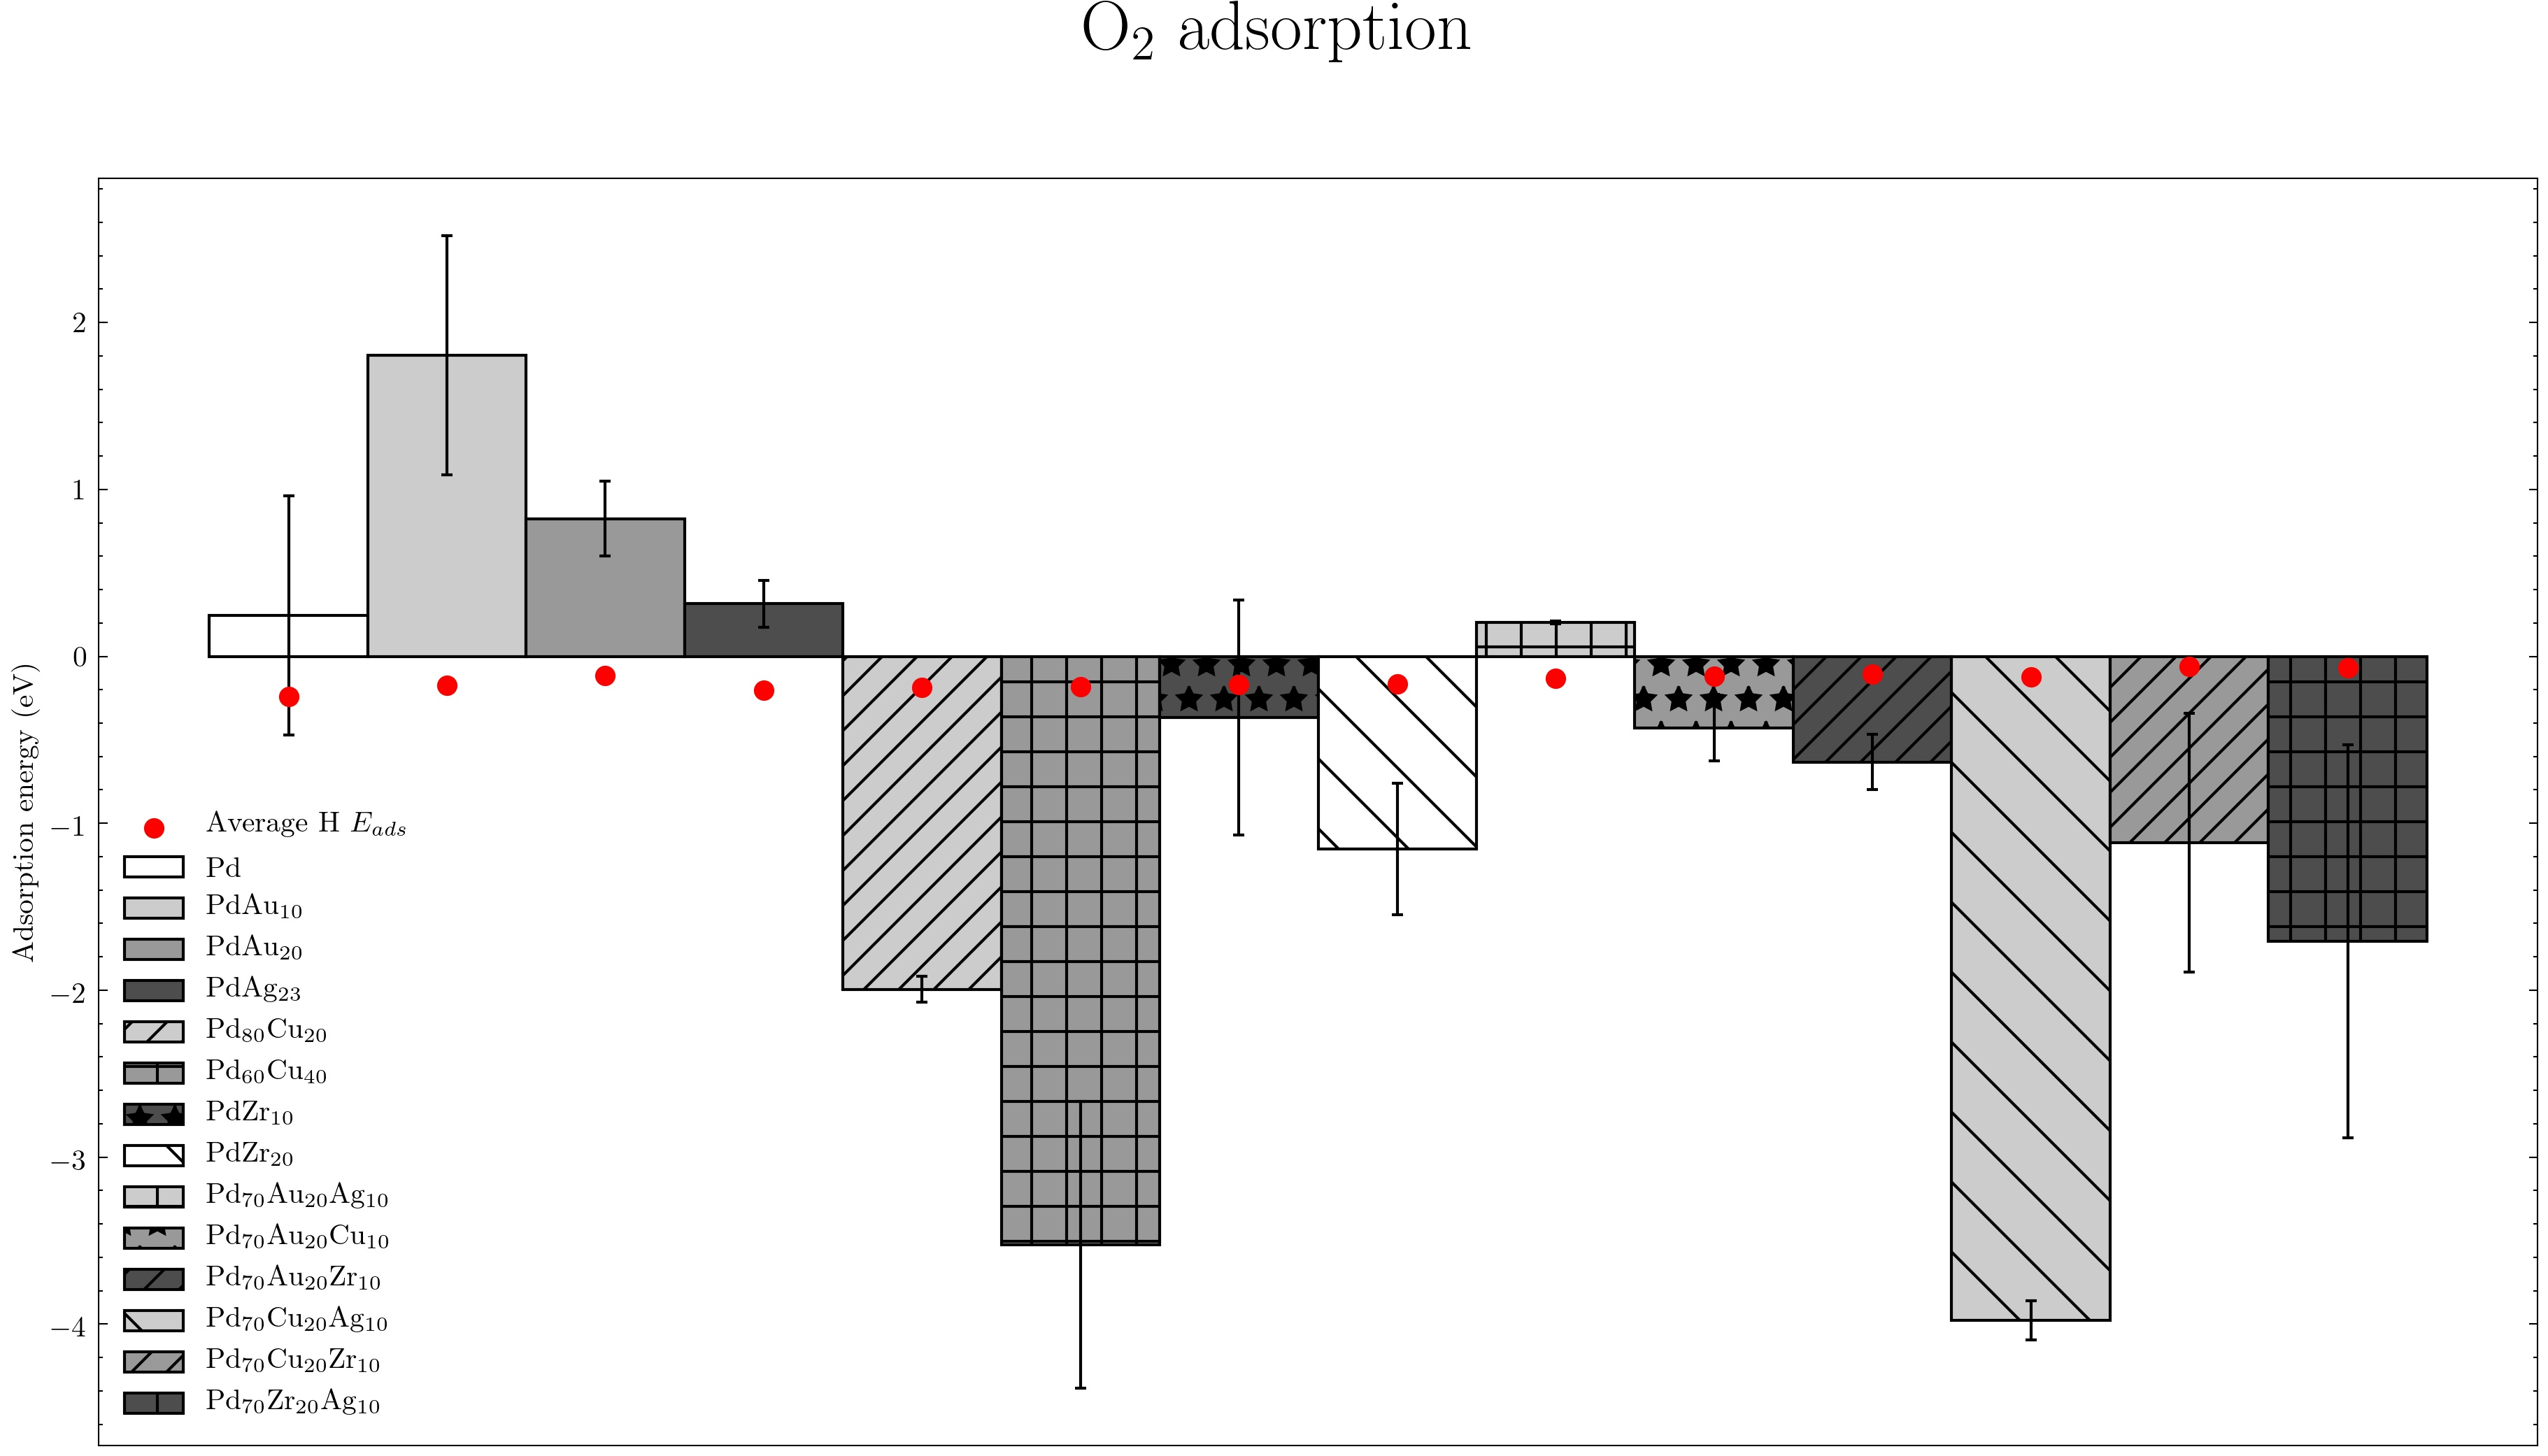
\includegraphics[width=0.9\linewidth,height=\textheight, keepaspectratio]{/Users/marc/Thesis/Chapter3/data/O2ads.jpg}
      \caption{Average adsorption energy of O\textsubscript{2} on the surface of palladium and palladium alloy slabs}
      \label{O2ads}
    \end{figure}
  
  \end{landscape}

\subsubsection{Water}

\begin{landscape}
  \begin{figure}
      \centering
      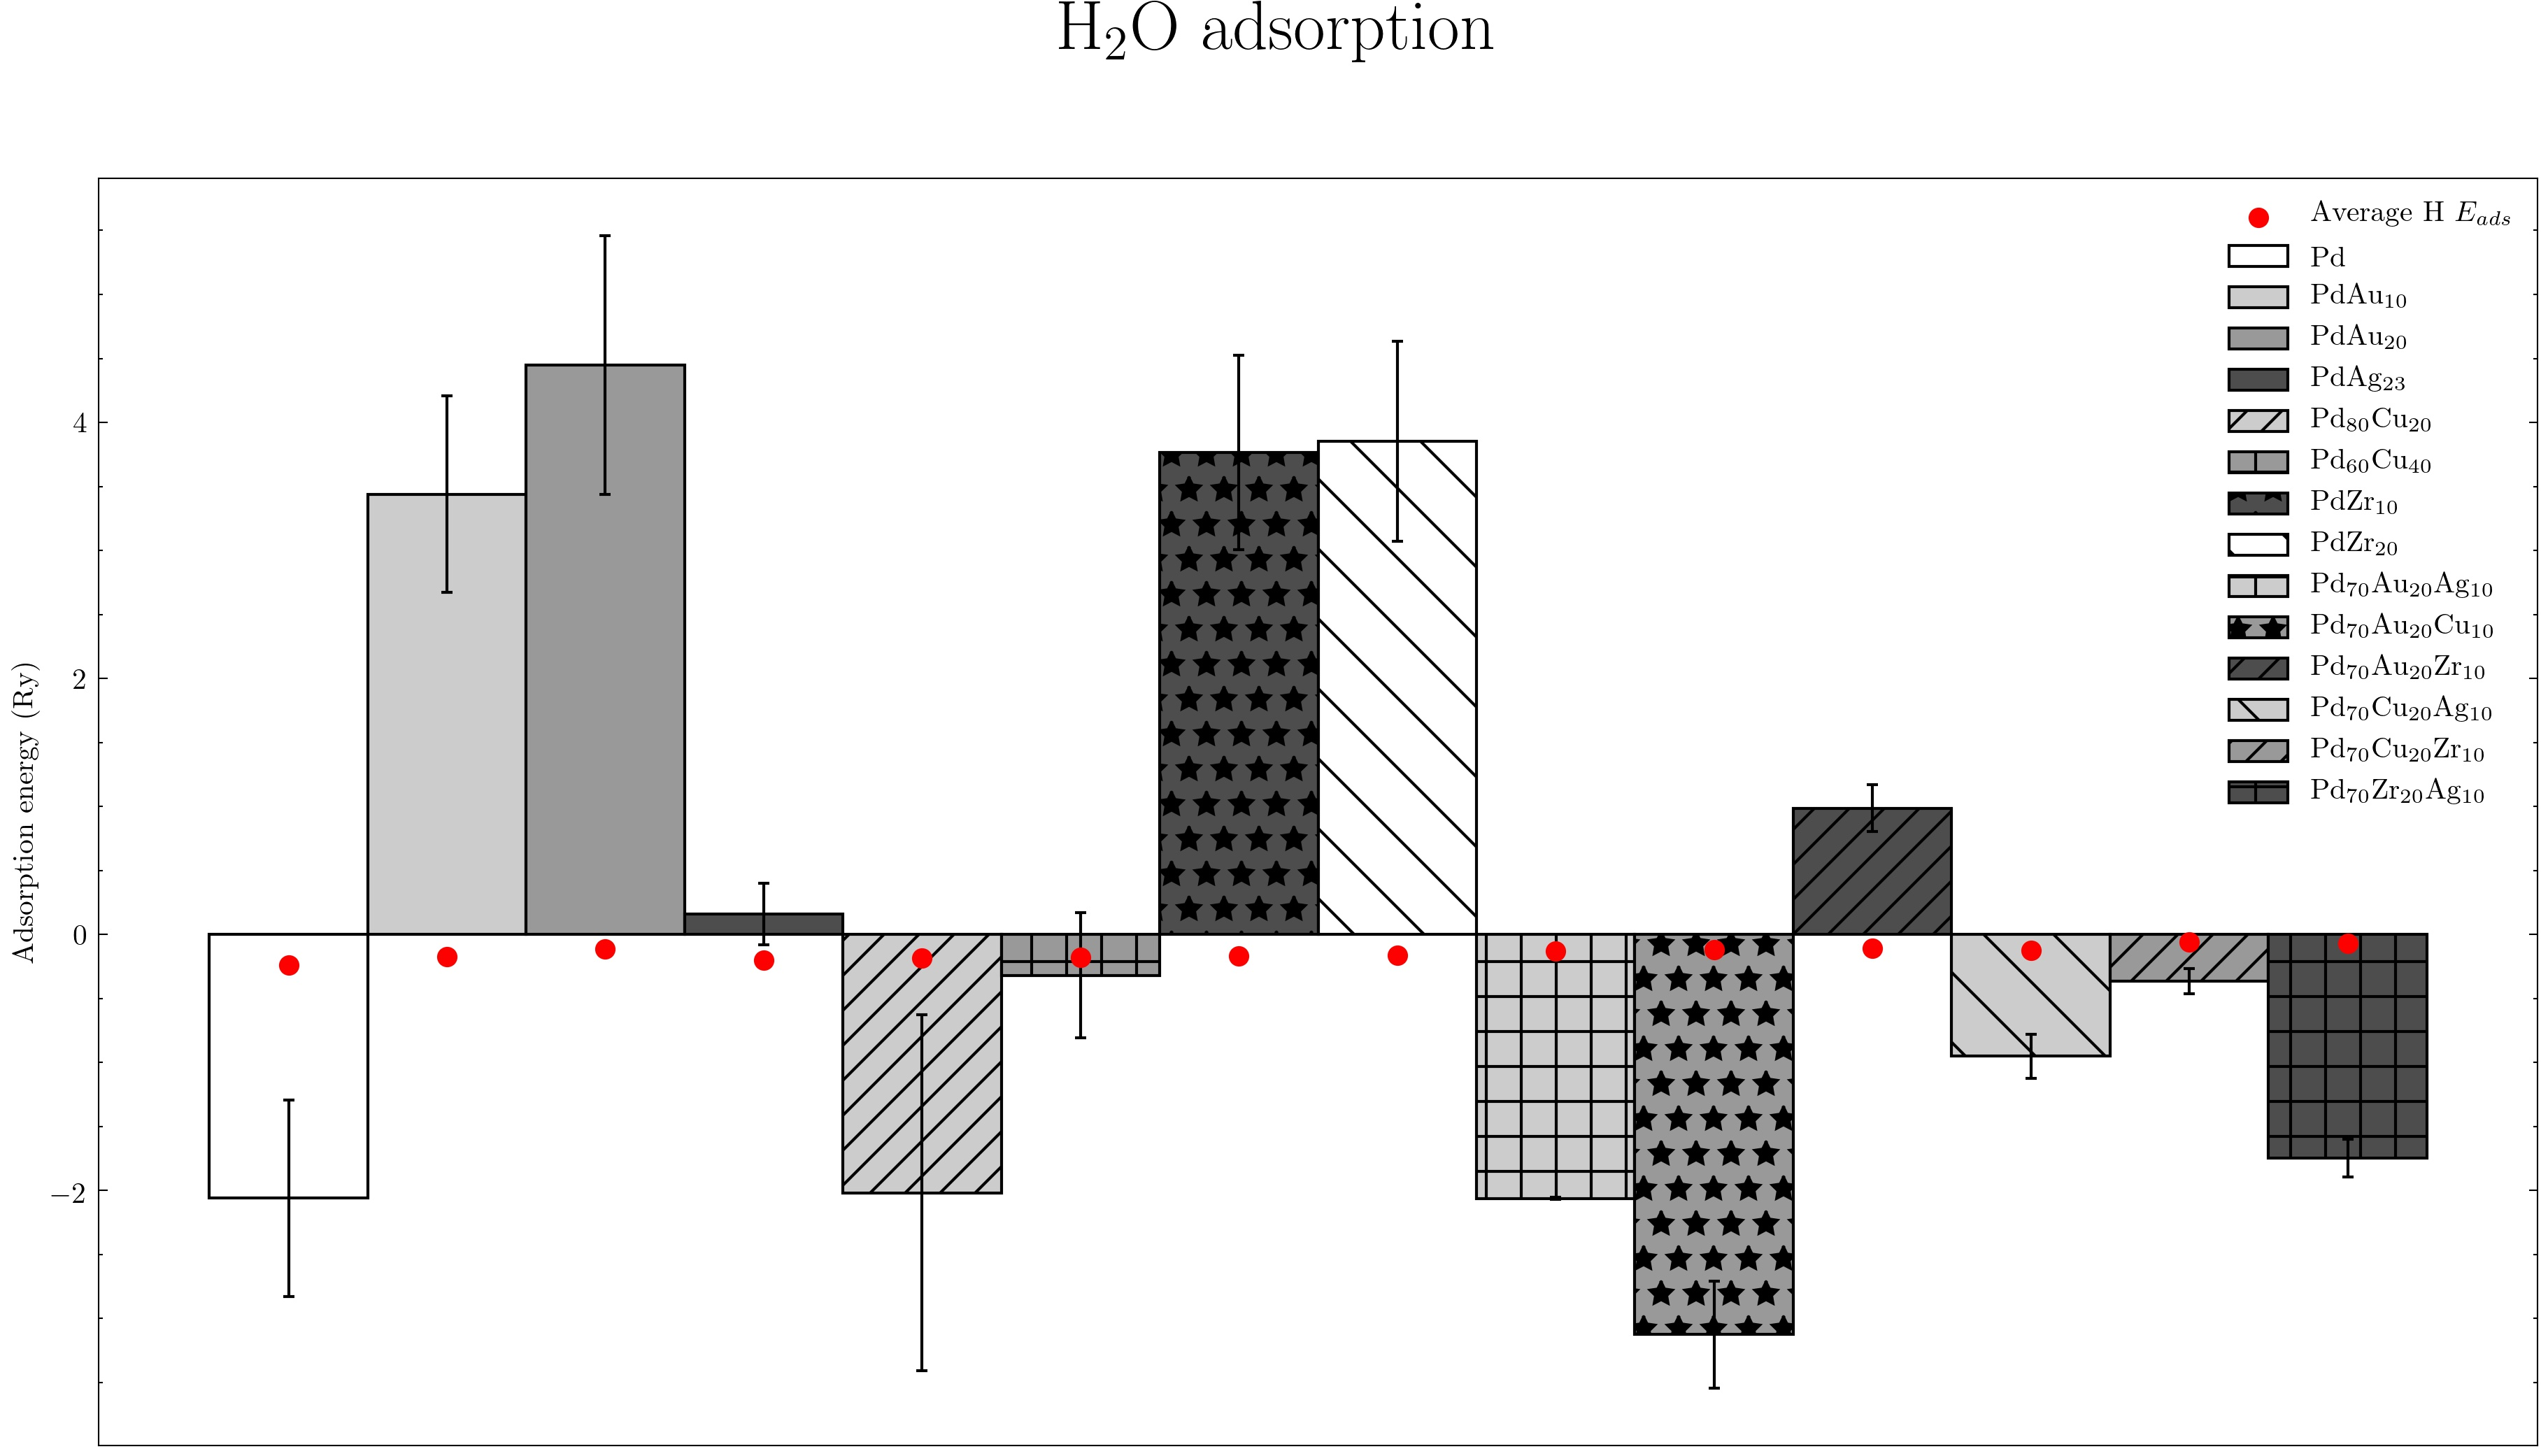
\includegraphics[width=0.9\linewidth,height=\textheight, keepaspectratio]{/Users/marc/Thesis/Chapter3/data/H2Oads.jpg}
      \caption{Average adsorption energy of H\textsubscript{2}O on the surface of palladium and palladium alloy slabs}
      \label{H2Oads}
    \end{figure}
  
  \end{landscape}
\subsubsection{Methane}
\begin{landscape}
  \begin{figure}
      \centering
      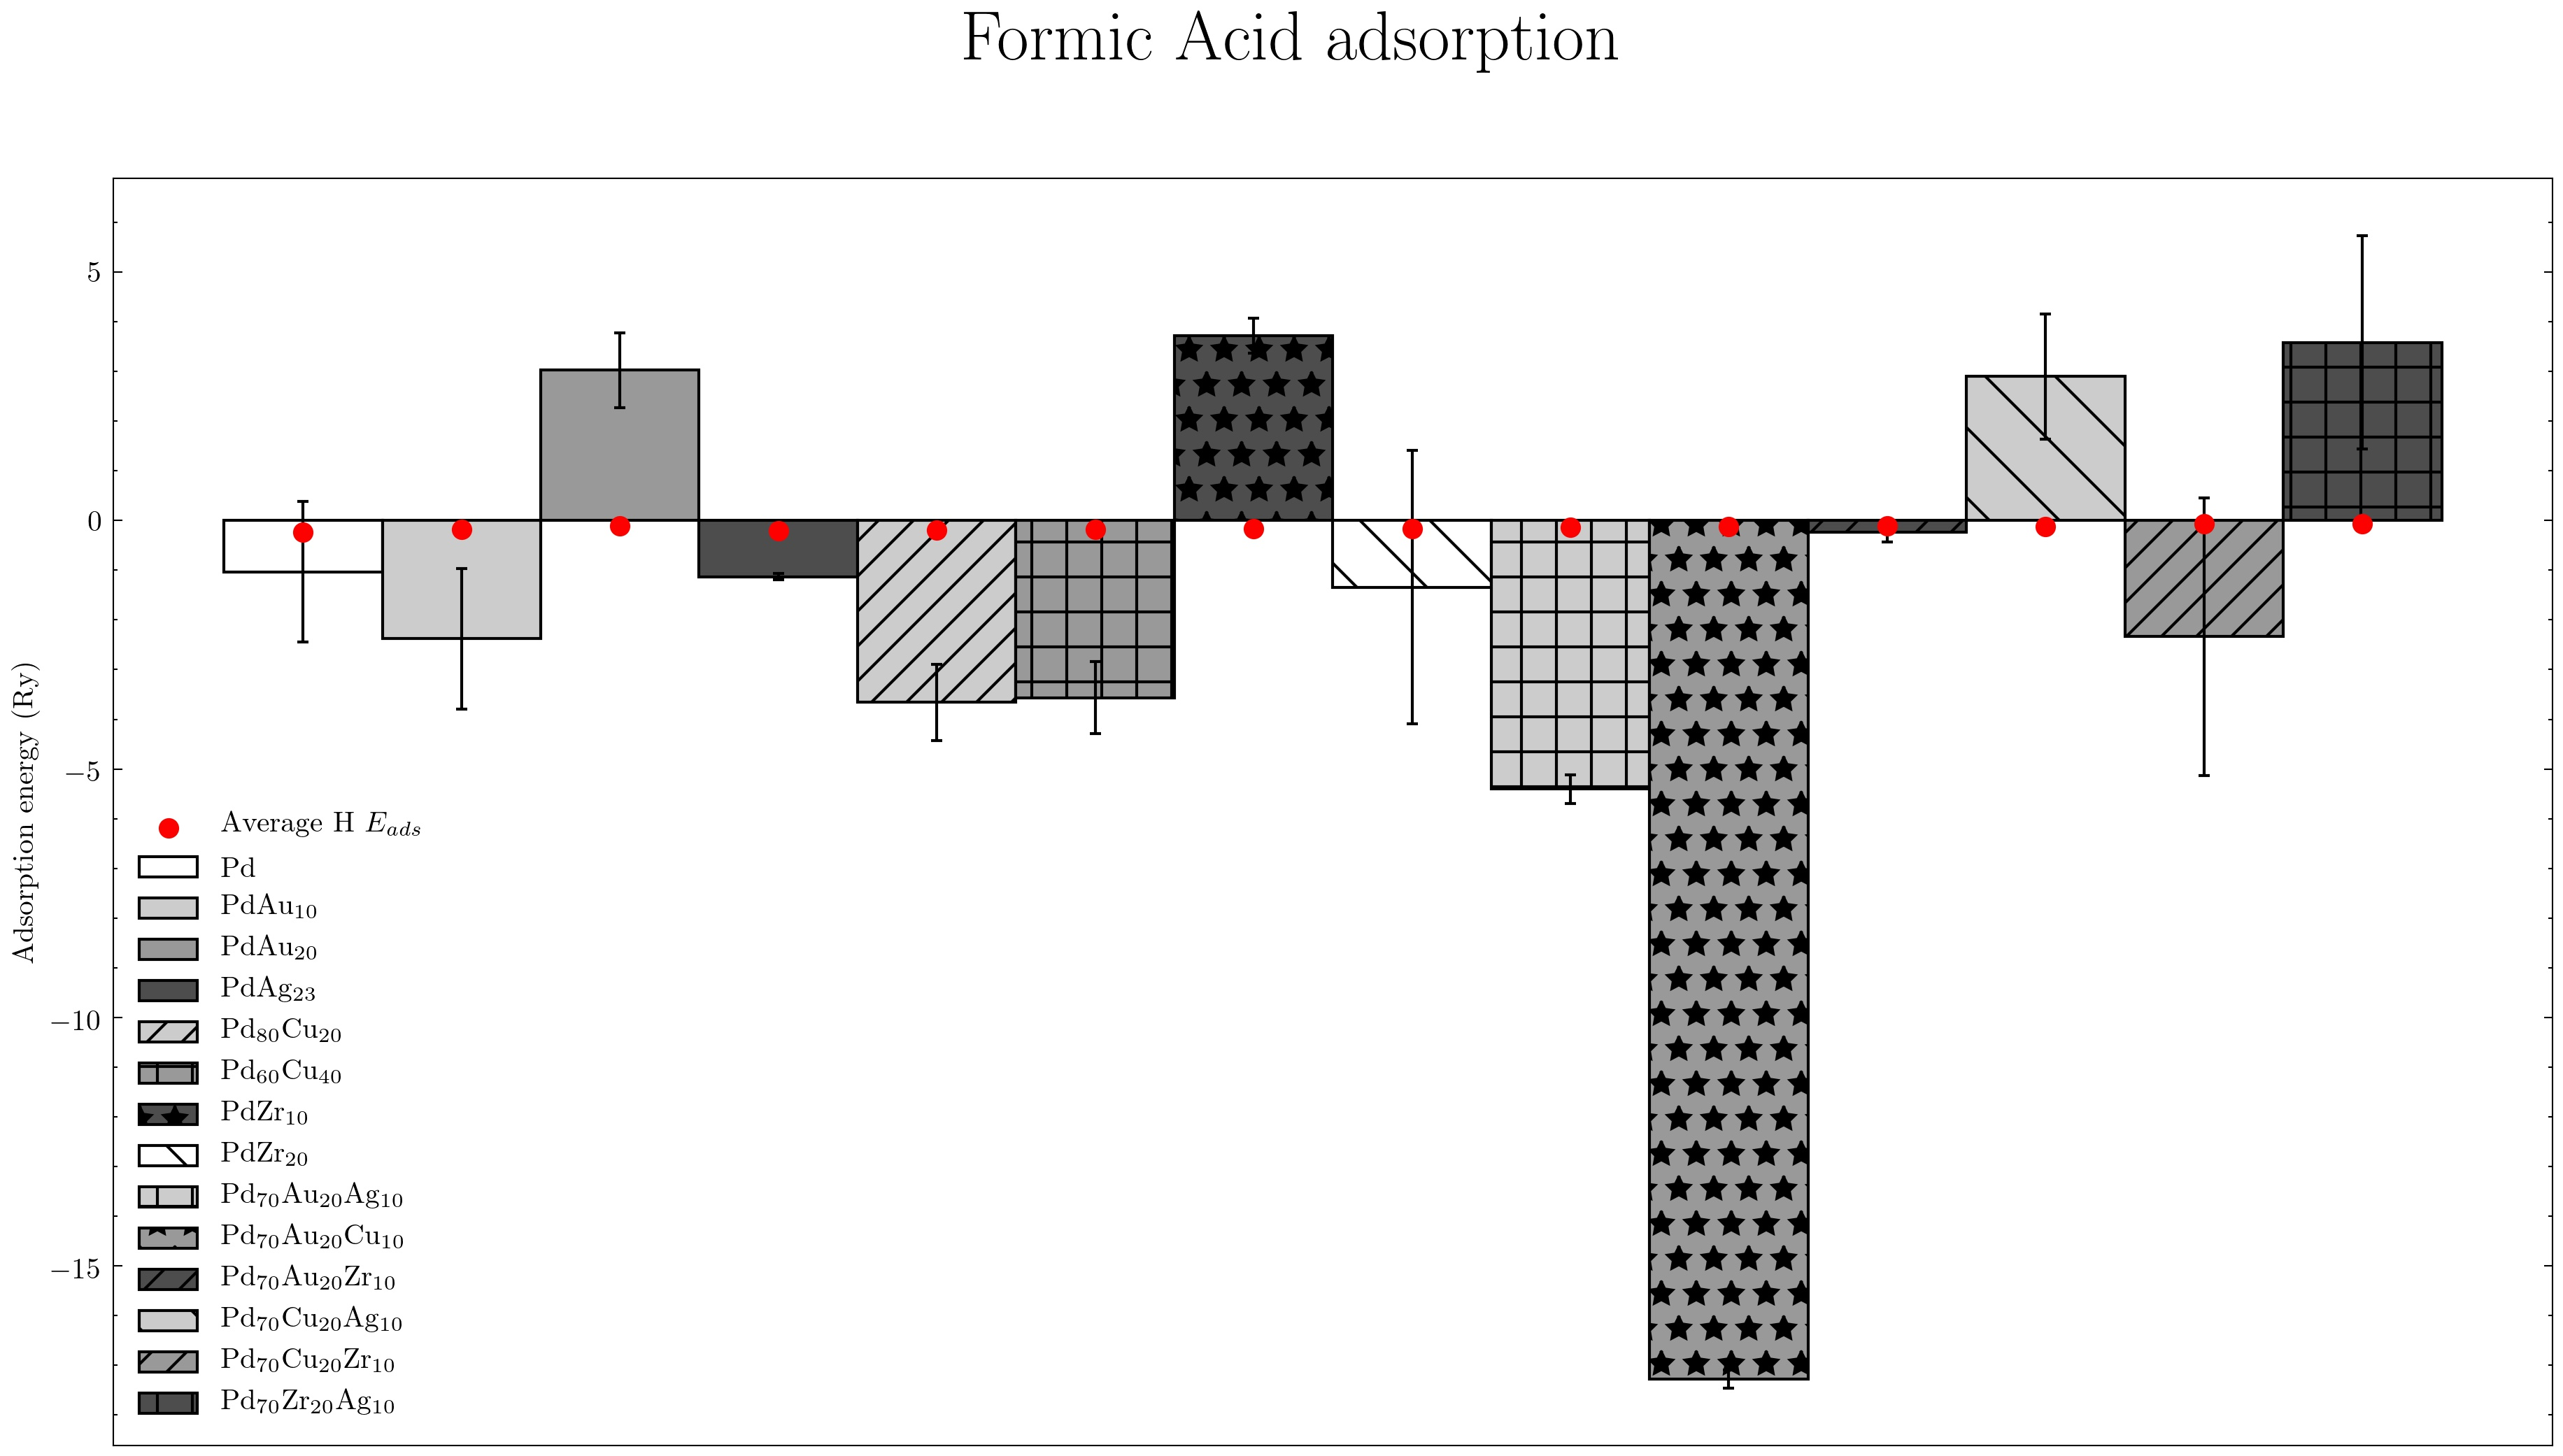
\includegraphics[width=0.9\linewidth,height=\textheight, keepaspectratio]{/Users/marc/Thesis/Chapter3/data/FAads.jpg}
      \caption{Average adsorption energy of Formic Acid on the surface of palladium and palladium alloy slabs}
      \label{CH4ads}
    \end{figure}
  
  \end{landscape}
\subsubsection{Formaldehyde}
\begin{landscape}
  \begin{figure}
      \centering
      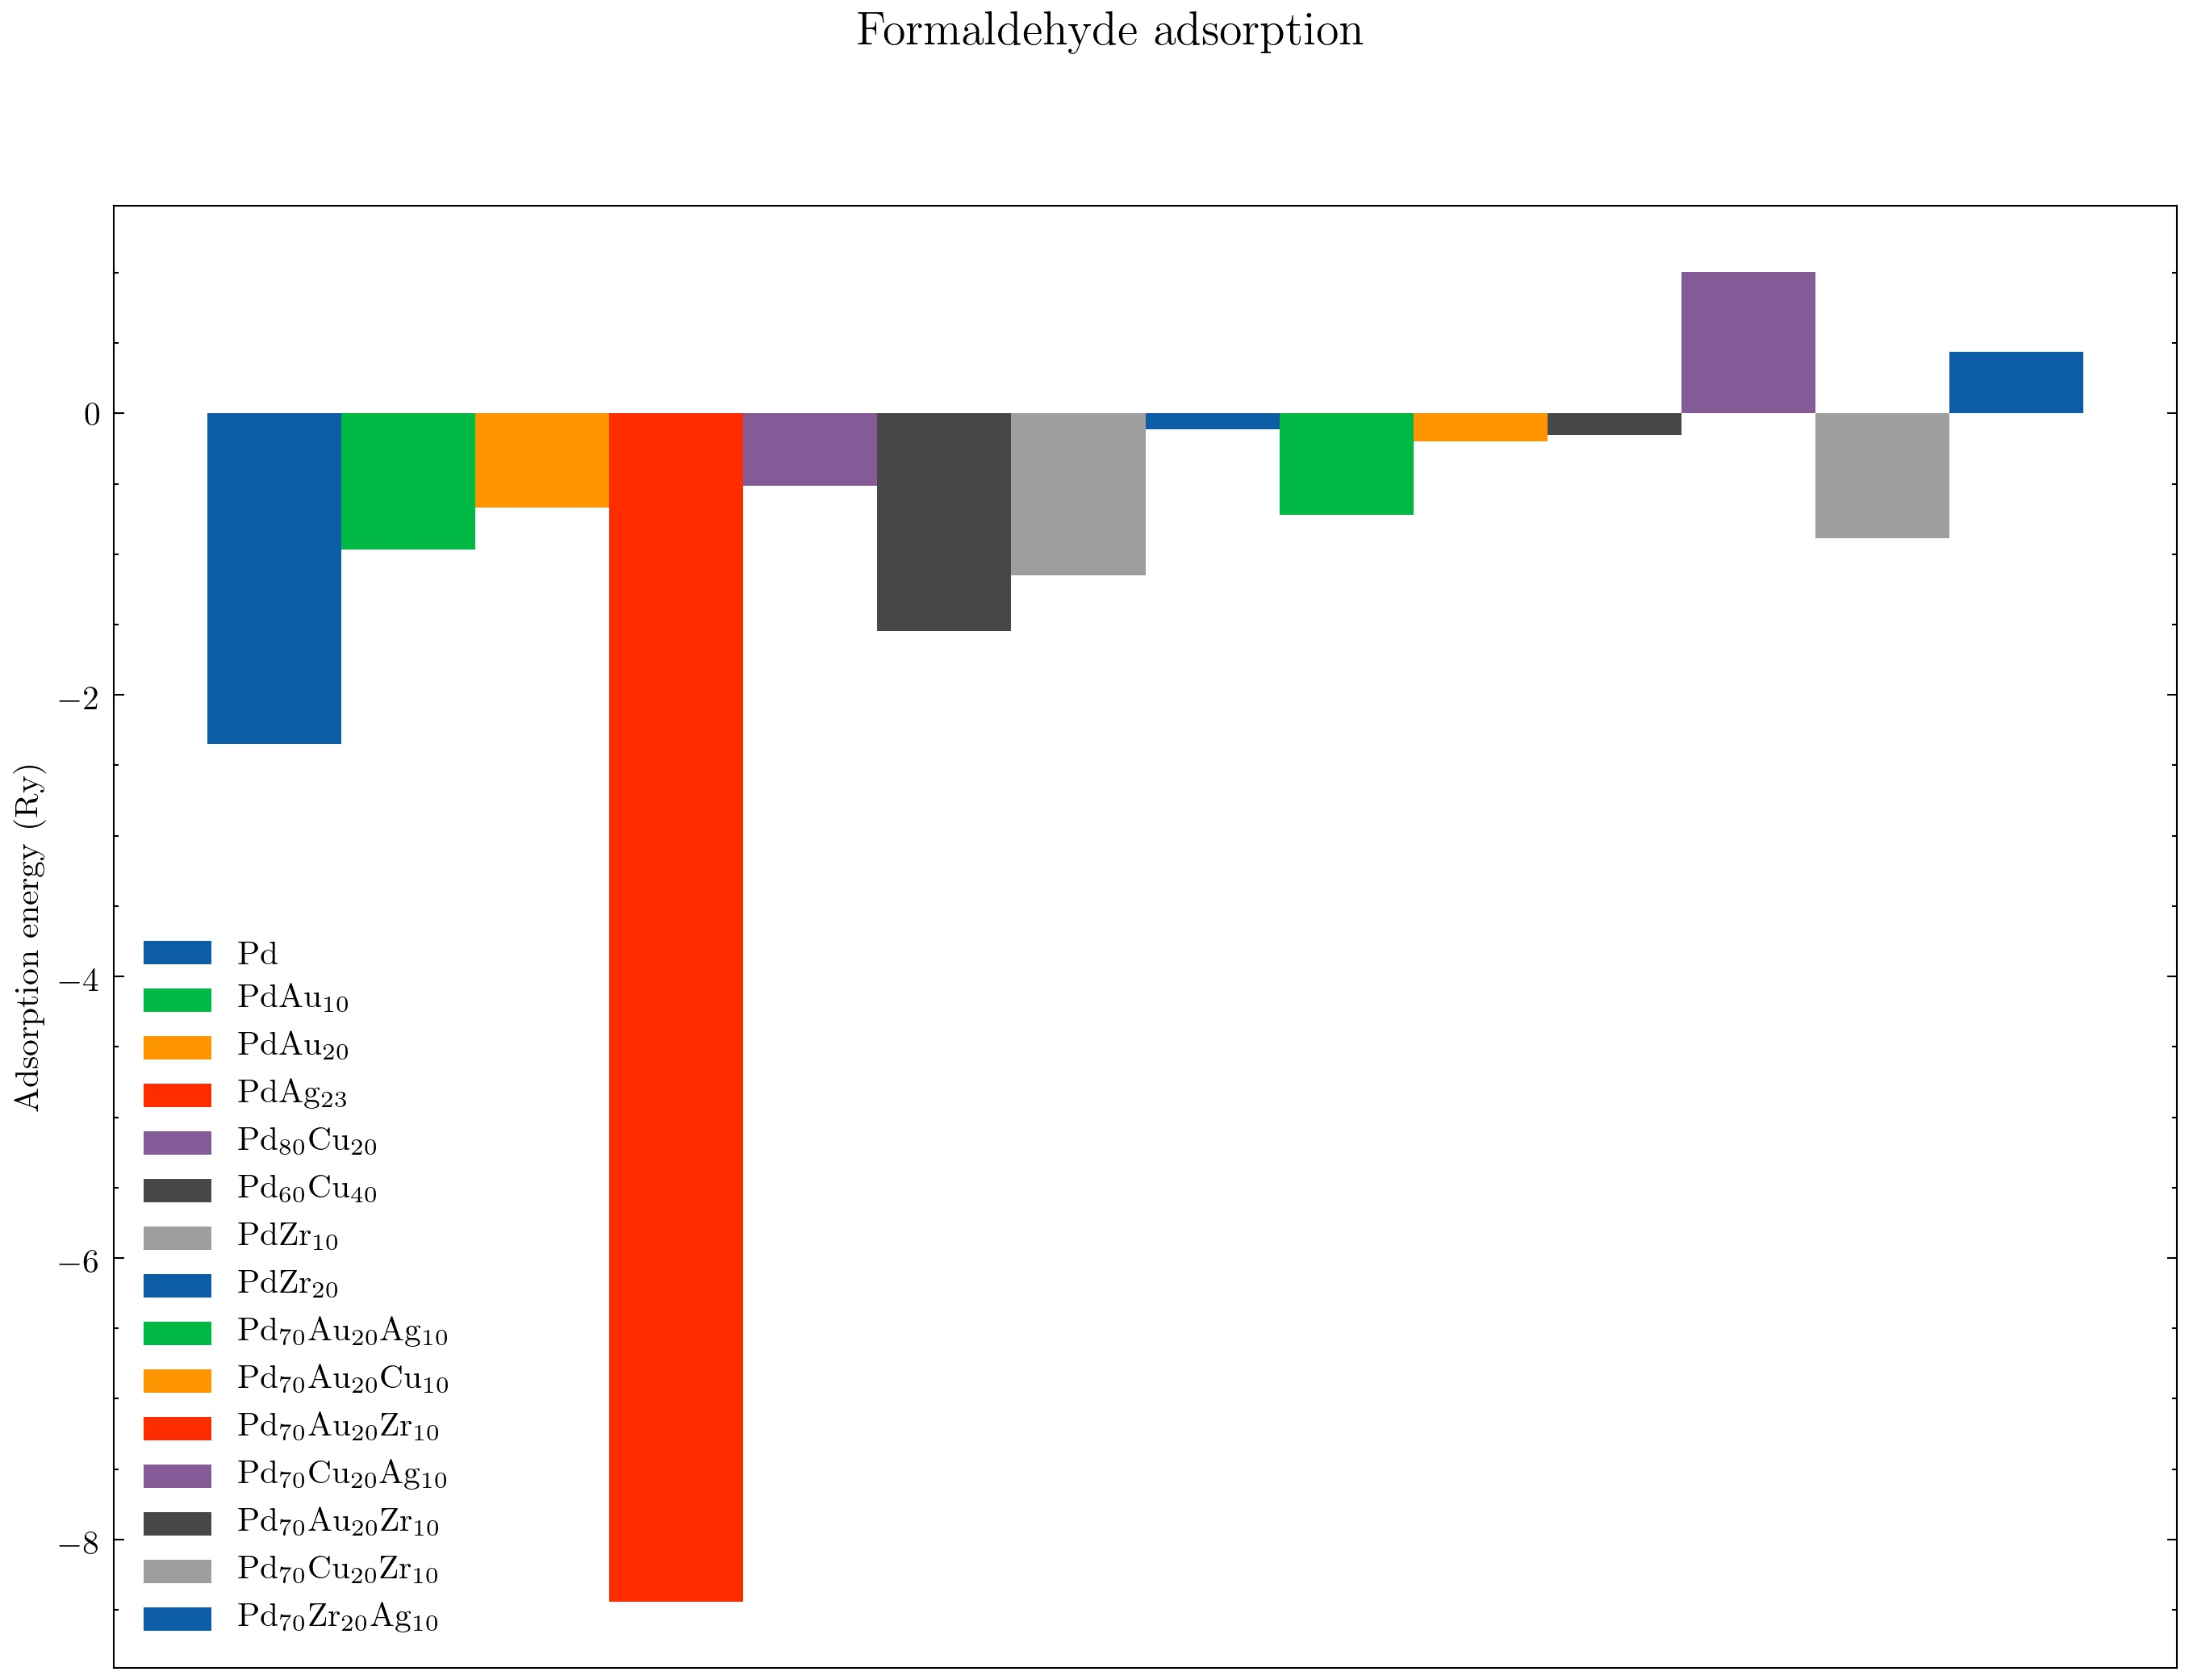
\includegraphics[width=0.9\linewidth,height=\textheight, keepaspectratio]{/Users/marc/Thesis/Chapter3/data/Formaldehydeads.jpg}
      \caption{Average adsorption energy of formaldehyde on the surface of palladium and palladium alloy slabs}
      \label{formaldehydeads}
    \end{figure}
  
  \end{landscape}

\subsubsection{Formic Acid}

\begin{landscape}
  \begin{figure}
      \centering
      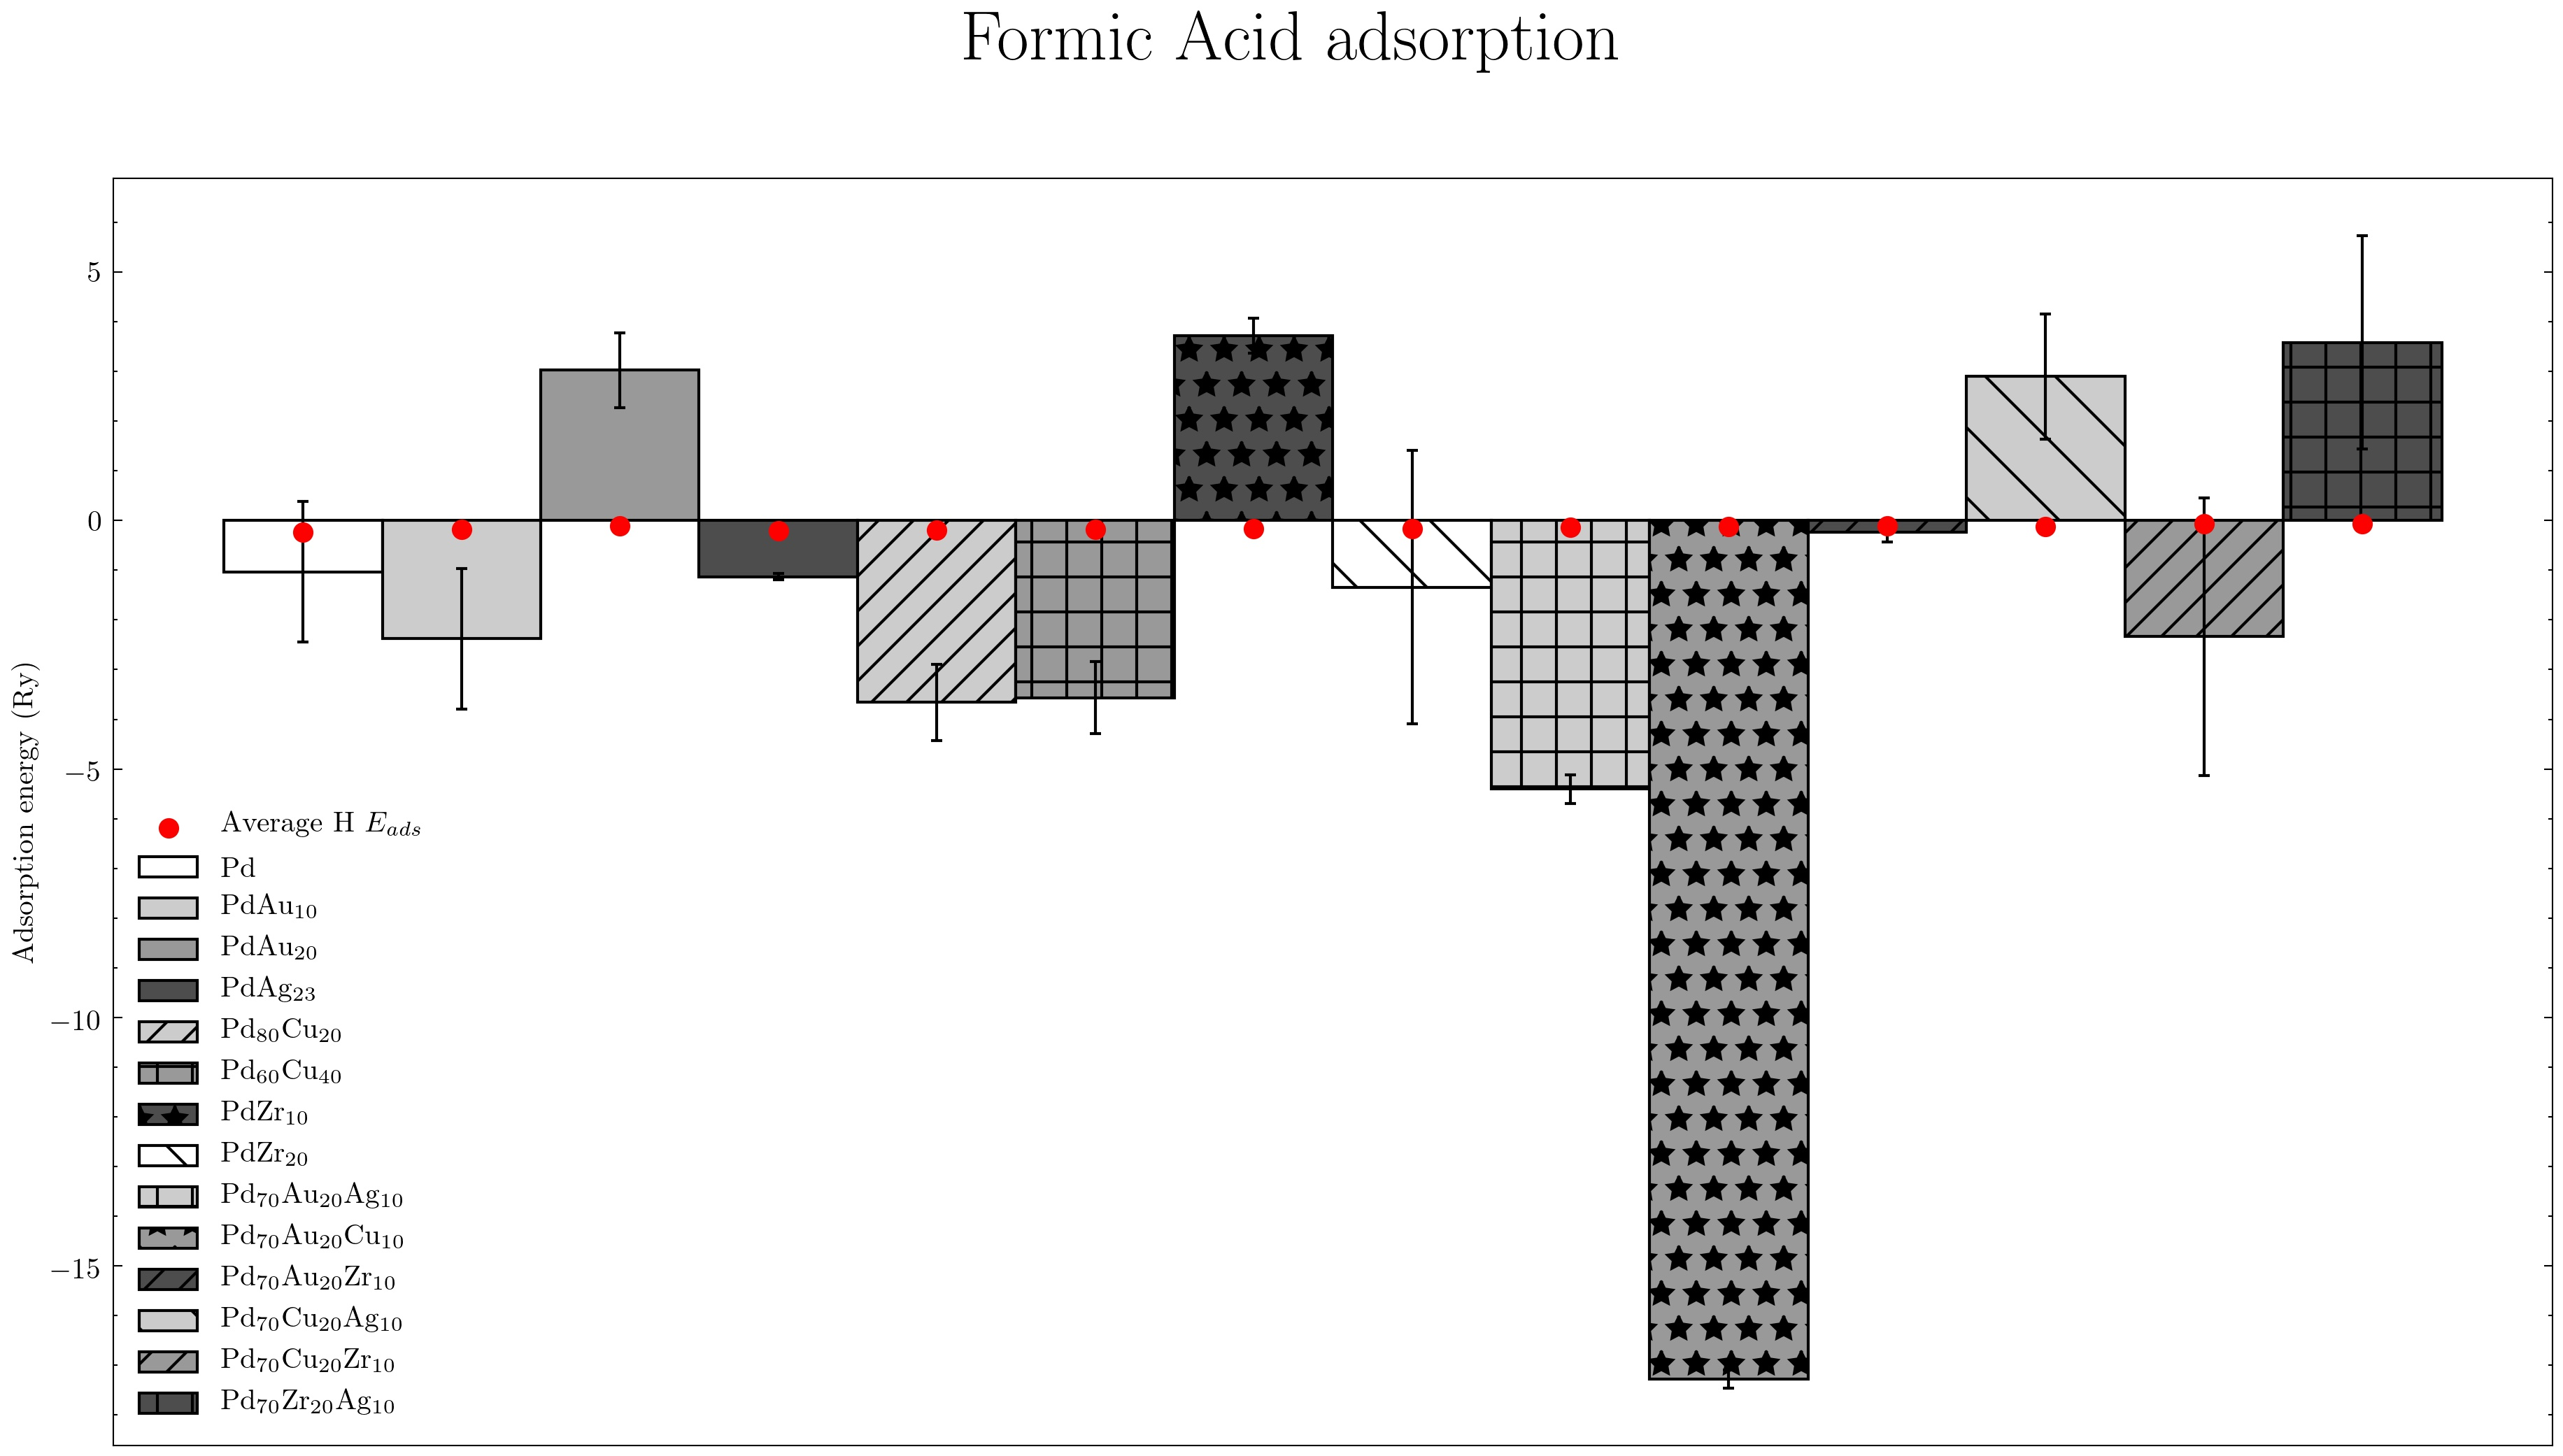
\includegraphics[width=0.9\linewidth,height=\textheight, keepaspectratio]{/Users/marc/Thesis/Chapter3/data/FAads.jpg}
      \caption{Average adsorption energy of Formic Acid on the surface of palladium and palladium alloy slabs}
      \label{FAads}
    \end{figure}
  
  \end{landscape}
\subsubsection{Hydrogen sulphide}
\begin{landscape}

\begin{figure}
    \centering
    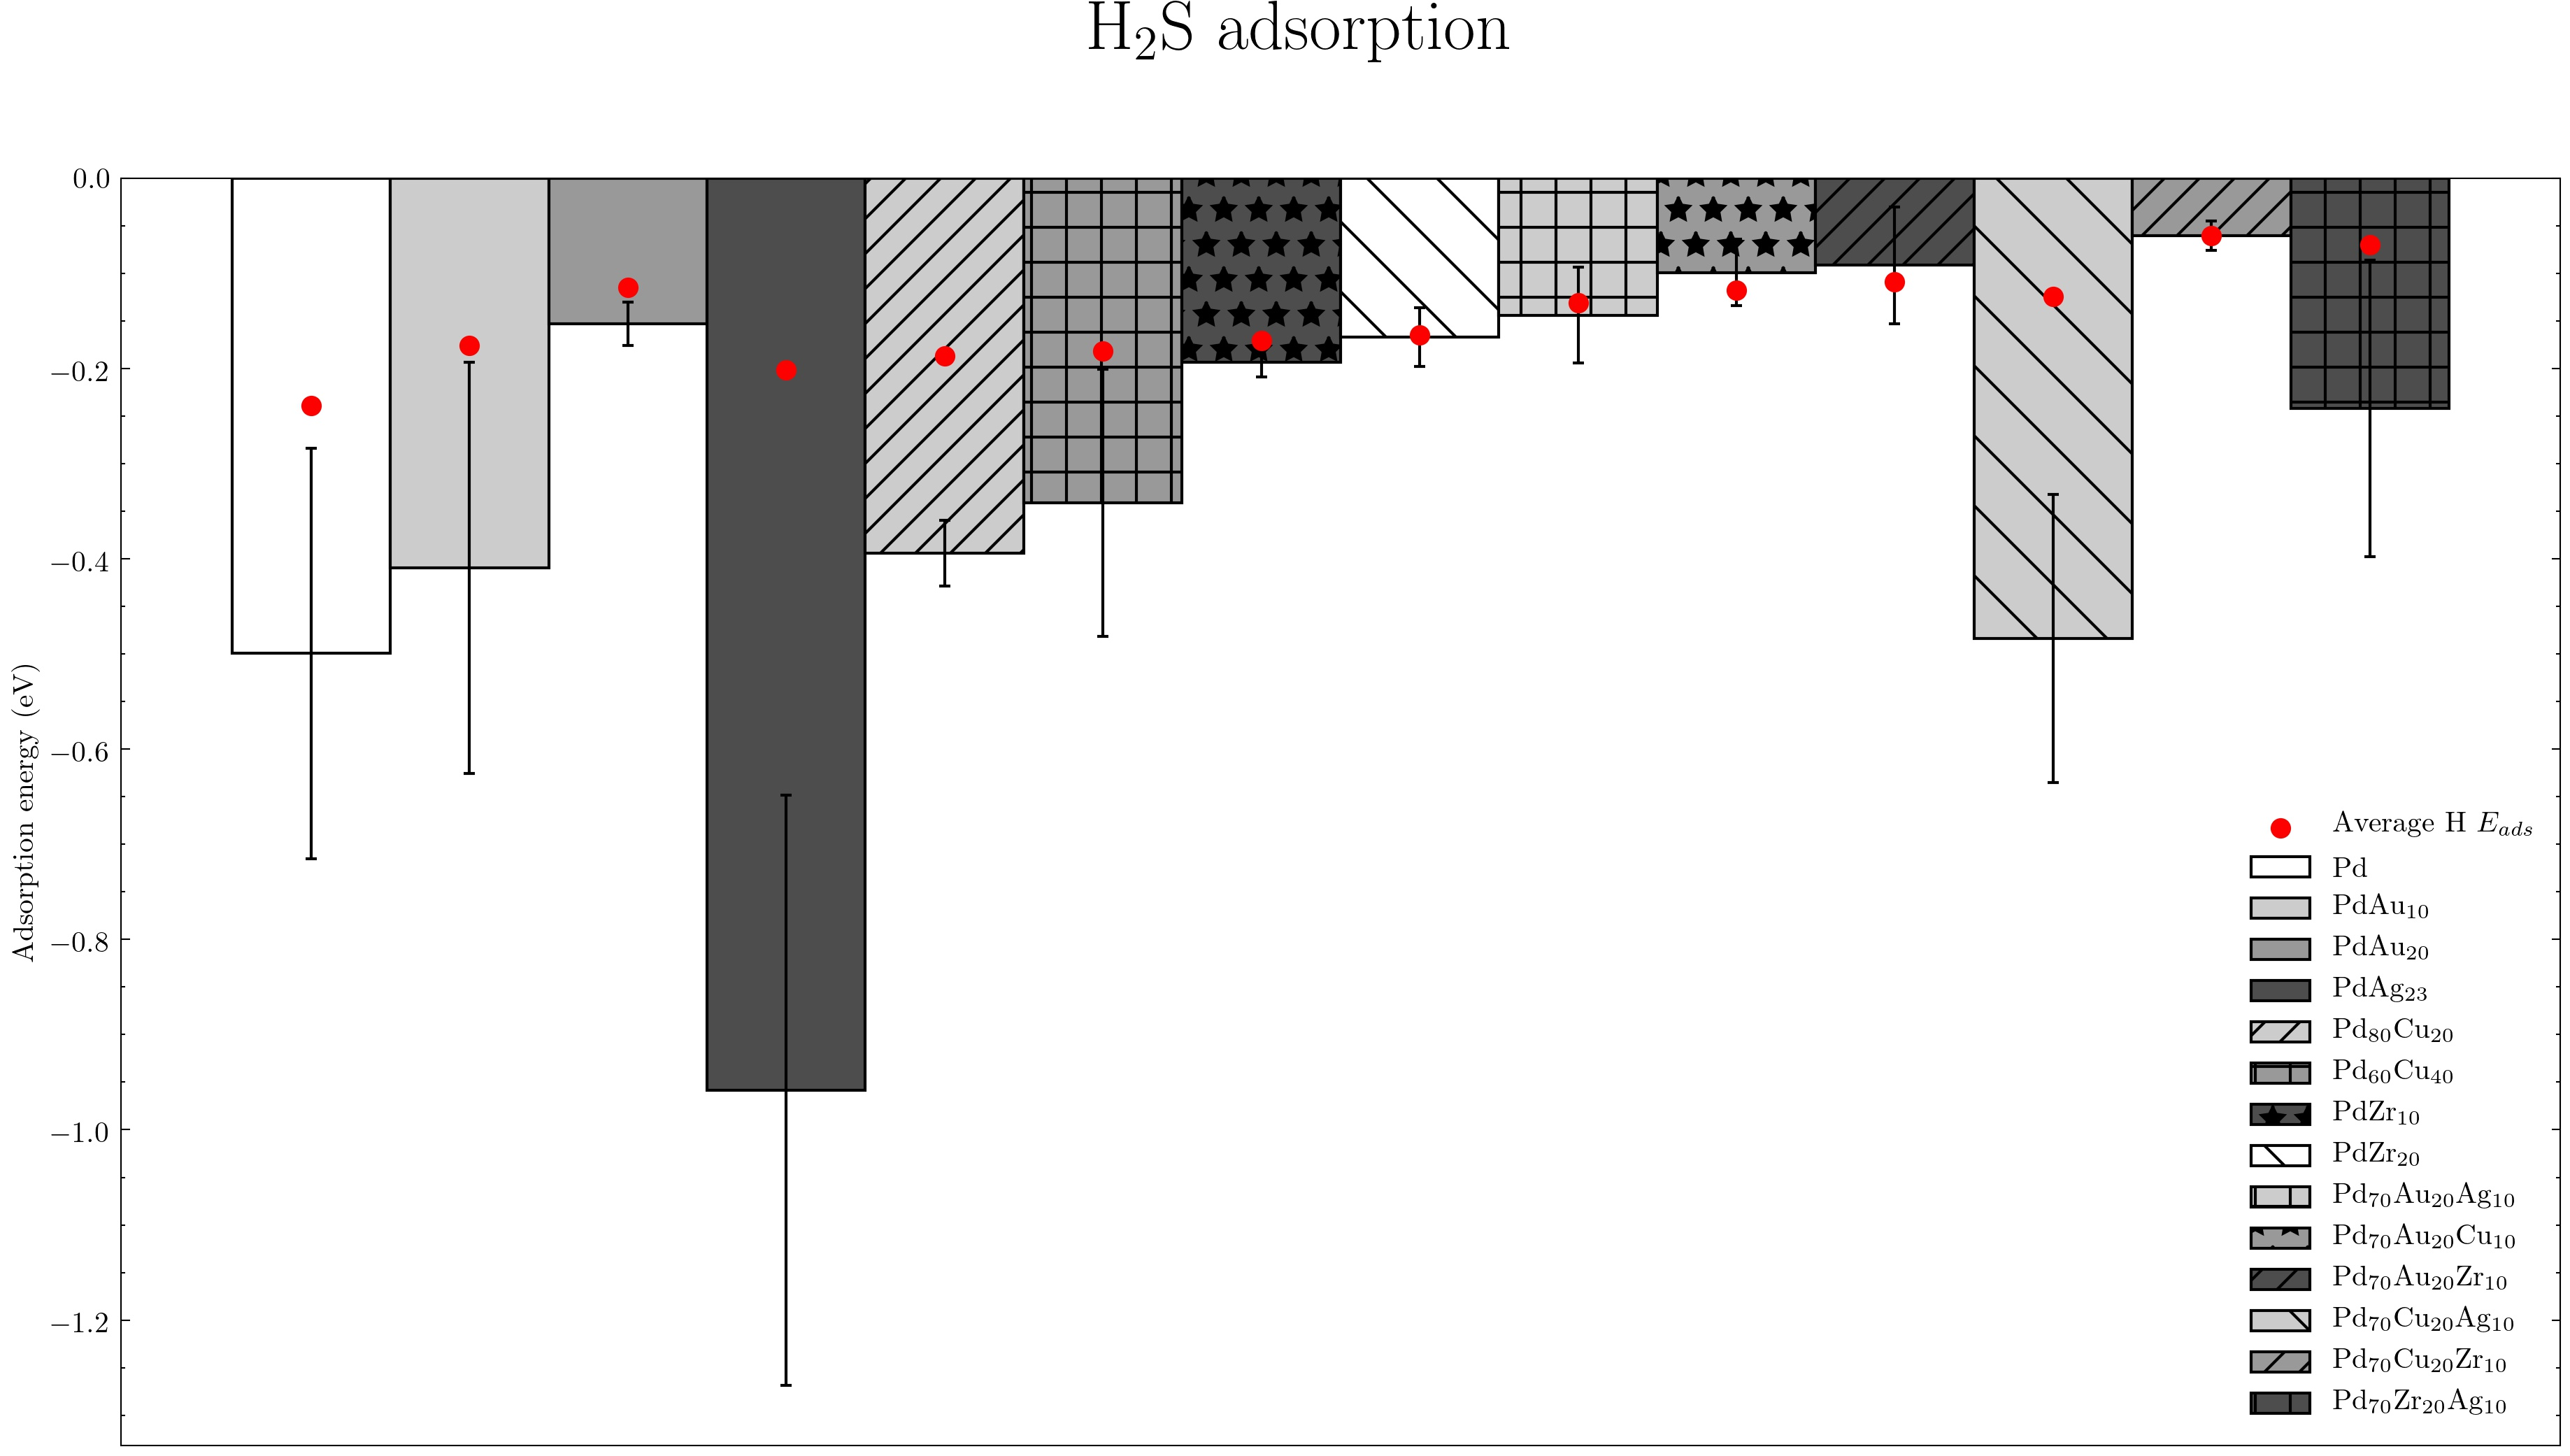
\includegraphics[width=0.9\linewidth,height=\textheight, keepaspectratio]{/Users/marc/Thesis/Chapter3/data/H2Sads.jpg}
    \caption{Average adsorption energy of H\textsubscript{2}S on the surface of palladium and palladium alloy slabs}
    \label{h2sads}
  \end{figure}
\end{landscape}


\section{Conclusion}
\bibliographystyle{plainnat}
\bibliography{library.bib}